\documentclass[aspectratio=169, 10pt]{beamer}

\usetheme[numbering=fraction, progressbar=frametitle]{metropolis}

\usepackage[T1]{fontenc}
\usepackage[utf8]{inputenc}
\usepackage[spanish,es-nodecimaldot]{babel}
\usepackage{tikz}
\usetikzlibrary{arrows.meta, shadows, shapes, positioning, calc, backgrounds, decorations.pathmorphing, fit}
\usepackage{booktabs}
\usepackage{siunitx}
\usepackage{graphicx}
\usepackage{array}
\usepackage{multicol}
\usepackage{subcaption}

% Paleta institucional UTN / Seguridad contra incendios
\definecolor{utnblue}{HTML}{003366}
\definecolor{utncyan}{HTML}{006699}
\definecolor{fireorange}{HTML}{E67E22}
\definecolor{firered}{HTML}{C0392B}
\definecolor{darkcharcoal}{HTML}{222831}
\definecolor{lightbg}{HTML}{FAFAFA}
\definecolor{cardbg}{HTML}{FFFFFF}
\definecolor{grayborder}{HTML}{DDDDDD}
\definecolor{successgreen}{HTML}{27AE60}
\definecolor{amberyellow}{HTML}{F39C12}

% Configuración de colores de Beamer
\setbeamercolor{normal text}{fg=darkcharcoal, bg=lightbg}
\setbeamercolor{frametitle}{fg=white, bg=utnblue}
\setbeamercolor{progress bar}{fg=fireorange, bg=utnblue!40}
\setbeamercolor{alerted text}{fg=firered}
\setbeamercolor{title separator}{fg=fireorange}

% Bloques personalizados
\setbeamercolor{block title}{bg=utnblue, fg=white}
\setbeamercolor{block body}{bg=utnblue!6, fg=darkcharcoal}
\setbeamercolor{block title alerted}{bg=firered, fg=white}
\setbeamercolor{block body alerted}{bg=firered!6, fg=darkcharcoal}
\setbeamercolor{block title example}{bg=utncyan, fg=white}
\setbeamercolor{block body example}{bg=utncyan!6, fg=darkcharcoal}

% Pie de página personalizado y continuo
\setbeamertemplate{footline}{%
  \leavevmode%
  \hbox{%
  \begin{beamercolorbox}[wd=.32\paperwidth,ht=2.4ex,dp=0.8ex,leftskip=0.8em]{footline}%
    \usebeamerfont{author in head/foot}\fontsize{5.5pt}{6.5pt}\selectfont\textbf{UTN-FRC} $\vert$ Higiene y Seguridad
  \end{beamercolorbox}%
  \begin{beamercolorbox}[wd=.50\paperwidth,ht=2.4ex,dp=0.8ex,center]{footline}%
    \usebeamerfont{title in head/foot}\fontsize{5.5pt}{6.5pt}\selectfont Prevención y Protección contra Incendios en Instalaciones
  \end{beamercolorbox}%
  \begin{beamercolorbox}[wd=.18\paperwidth,ht=2.4ex,dp=0.8ex,rightskip=0.8em]{footline}%
    \usebeamerfont{date in head/foot}\hfill\fontsize{5.5pt}{6.5pt}\selectfont\insertframenumber{} / \inserttotalframenumber
  \end{beamercolorbox}}%
  \vskip0pt%
}
\setbeamercolor{footline}{bg=lightbg!80!black, fg=darkcharcoal}

% Unidades y macros
\newcommand{\m}{\,\mathrm{m}}
\newcommand{\mm}{\,\mathrm{mm}}
\newcommand{\kg}{\,\mathrm{kg}}
\newcommand{\Celsius}{^\circ\mathrm{C}}
\newcommand{\percent}{\%}

\title[Prevención y Protección contra Incendios]{Prevención y Protección contra Incendios en Instalaciones Industriales y Electrónicas}
\subtitle{Trabajo Práctico Final --- Cátedra de Seguridad, Higiene y Medio Ambiente}
\author{Ignacio Gil \and Gaston Grasso \and Franco Palombo \and Angelo Prieto}
\institute{Universidad Tecnológica Nacional --- Facultad Regional Córdoba}
\date{Comisión 4R2 --- Ciclo Lectivo 2026}
\titlegraphic{\hfill
\includegraphics[height=1.0cm]{images/UTN_logo.png}}

\begin{document}

% --- PORTADA ---
\begin{frame}[plain]
  \titlepage
\end{frame}

% --- AGENDA CONTINUA ---
\begin{frame}{Estructura y Hoja de Ruta de la Exposición}
  \begin{columns}[T]
    \begin{column}{0.48\textwidth}
      \begin{block}{\textbf{I. Fundamentos Físicos y Química del Fuego}}
        \scriptsize
        $\bullet$ Fuego vs. Incendio y principios de reacción.\\
        $\bullet$ Modelos del Triángulo y Tetraedro del Fuego.\\
        $\bullet$ Curva temporal de desarrollo y \textit{flashover}.\\
        $\bullet$ Regímenes de combustión (deflagración vs. detonación).\\
        $\bullet$ Límites de inflamabilidad y clasificación A-B-C-D-K.
      \end{block}
      \vspace{0.2cm}
      \begin{block}{\textbf{II. Toxicología, Humos y Marco Legal}}
        \scriptsize
        $\bullet$ Toxicología de gases asfixiantes ($CO, HCN$) e irritantes.\\
        $\bullet$ Dinámica del humo, plano neutro y colores diagnósticos.\\
        $\bullet$ Ley 19.587 y Decreto 351/79 (Anexo VII).\\
        $\bullet$ Carga de fuego ($Q_f$), medios de escape (UAS) y AEA 90364.
      \end{block}
    \end{column}

    \begin{column}{0.48\textwidth}
      \begin{block}{\textbf{III. Tecnologías de Detección y Extinción}}
        \scriptsize
        $\bullet$ Topologías convencionales vs. direccionables en anillo.\\
        $\bullet$ Sensores ópticos (Tyndall), iónicos ($^{241}\mathrm{Am}$) y ASD/VESDA.\\
        $\bullet$ Extintores portátiles: agentes, rating y descarga de $CO_2$.\\
        $\bullet$ Sistemas fijos: Redes de hidrantes (R.I.A.) y rociadores.
      \end{block}
      \vspace{0.2cm}
      \begin{block}{\textbf{IV. Prevención, Protección y Casos Reales}}
        \scriptsize
        $\bullet$ Jerarquía de control de riesgos y tipos de protección.\\
        $\bullet$ Sustitución por ésteres dieléctricos, AFDD y termografía.\\
        $\bullet$ Protocolos operativos (LOTO, PTC) y protección pasiva ($F$).\\
        $\bullet$ Organización de brigadas (E.P.I. y E.S.I.) y casos forenses.
      \end{block}
    \end{column}
  \end{columns}
\end{frame}

% =============================================================================
% PARTE I: FUNDAMENTOS FÍSICOS, CINÉTICA Y QUÍMICA DEL FUEGO
% =============================================================================

% --- SLIDE 3: FUEGO VS INCENDIO ---
\begin{frame}{Fuego frente a Incendio}
  \begin{columns}[T]
    \begin{column}{0.48\textwidth}
      \begin{block}{\textbf{Fuego}}
        \small
        $\bullet$ Reacción fisicoquímica de óxido-reducción fuertemente exotérmica.\\
        $\bullet$ Emisión de luz, calor y humos.\\
        $\bullet$ \textbf{Condición operativa:} Parámetros espaciales, temporales y de combustible están gobernados por el ser humano.
      \end{block}
      \vspace{0.2cm}
      \centering
      \resizebox{0.9\columnwidth}{!}{%
        \begin{tikzpicture}
          \node[draw=successgreen!80!black, fill=successgreen!10, rounded corners=4pt, line width=1.2pt, inner sep=6pt, text width=5cm, align=center] {
            \textbf{Energía Aprovechable}\\[2pt]
            \scriptsize Hornos $\cdot$ Calderas
          };
        \end{tikzpicture}
      }
    \end{column}

    \begin{column}{0.48\textwidth}
      \begin{alertblock}{\textbf{Incendio (Siniestro Descontrolado)}}
        \small
        $\bullet$ Fuego que escapa a las barreras de contención.\\
        $\bullet$ Se propaga \textbf{sin control en el tiempo ni en el espacio}.\\
        $\bullet$ Destrucción de estructuras, ruina de activos y riesgo severo para la integridad de los operarios.
      \end{alertblock}
      \vspace{0.2cm}
      \centering
      \resizebox{0.9\columnwidth}{!}{%
        \begin{tikzpicture}
          \node[draw=firered!80!black, fill=firered!10, rounded corners=4pt, line width=1.2pt, inner sep=6pt, text width=5cm, align=center] {
            \textbf{Siniestro Destructivo}\\[2pt]
            \scriptsize Colapso edilicio $\cdot$ Gases letales $\cdot$ Pérdidas humanas
          };
        \end{tikzpicture}
      }
    \end{column}
  \end{columns}
\end{frame}

% --- SLIDE 4: TRIÁNGULO DEL FUEGO ---
\begin{frame}{Modelo Clásico: El Triángulo del Fuego}
  \begin{columns}[c]
    \begin{column}{0.48\textwidth}
      \small
      Para que exista combustión deben converger tres elementos simultáneos:
      \begin{enumerate}
        \scriptsize
        \item \textbf{Combustible:} Sustancia reductora susceptible de oxidarse (sólido, líquido o gas).
        \item \textbf{Comburente:} Agente oxidante ($O_2$ del aire; requiere concentración $\ge 14\text{--}15\%$).
        \item \textbf{Calor / Energía de activación:} Aporte térmico para alcanzar la temperatura de ignición.
      \end{enumerate}
      \vspace{0.15cm}
      \begin{alertblock}{\textbf{Mecanismos Clásicos de Extinción}}
        \scriptsize
        $\bullet$ \textbf{Desalimentación:} Supresión física del combustible.\\
        $\bullet$ \textbf{Sofocación:} Aislamiento o desplazamiento del $O_2$.\\
        $\bullet$ \textbf{Enfriamiento:} Disipación de calor por debajo del punto de ignición.
      \end{alertblock}
    \end{column}

    \begin{column}{0.50\textwidth}
      \centering
      \resizebox{0.95\columnwidth}{!}{%
        \begin{tikzpicture}[scale=0.9, line join=round, line cap=round]
          \definecolor{cCalor}{RGB}{205, 35, 25}
          \definecolor{cComb}{RGB}{30, 135, 50}
          \definecolor{cOx}{RGB}{20, 100, 190}

          \coordinate (A) at (0, 2.0);
          \coordinate (B) at (-2.1, -1.0);
          \coordinate (C) at (2.1, -1.0);

          \fill[yellow!12] (A) -- (B) -- (C) -- cycle;

          \draw[cComb!90!black, line width=3.5pt] (A) -- node[left=2pt, font=\bfseries\small, cComb!90!black]{Combustible} (B);
          \draw[cOx!90!black, line width=3.5pt] (A) -- node[right=2pt, font=\bfseries\small, cOx!90!black]{Comburente ($O_2$)} (C);
          \draw[cCalor!90!black, line width=3.5pt] (B) -- node[below=2pt, font=\bfseries\small, cCalor!90!black]{Calor (Activación)} (C);

          \begin{scope}[shift={(0, -0.15)}, scale=0.55]
            \shade[inner color=yellow!90!white, outer color=orange!95!red, opacity=0.9]
              (0,-0.6) .. controls (-0.7,-0.2) and (-0.6,0.6) .. (0,1.4)
                       .. controls (0.6,0.6) and (0.7,-0.2) .. (0,-0.6);
            \shade[inner color=white, outer color=yellow!85!orange, opacity=0.95]
              (0,-0.4) .. controls (-0.35,-0.1) and (-0.3,0.3) .. (0,0.8)
                       .. controls (0.3,0.3) and (0.35,-0.1) .. (0,-0.4);
          \end{scope}
        \end{tikzpicture}
      }
    \end{column}
  \end{columns}
\end{frame}

% --- SLIDE 5: TETRAEDRO DEL FUEGO ---
\begin{frame}{Evolución Teórica: El Tetraedro del Fuego}
  \begin{columns}[c]
    \begin{column}{0.48\textwidth}
      \small
      En la combustión viva con llama no basta con la presencia simultánea de combustible, oxígeno y calor.
      \begin{block}{\textbf{El Cuarto Elemento: Reacción en Cadena}}
        \scriptsize
        $\bullet$ La combustión se autosostiene mediante radicales libres intermedios altamente inestables ($H^\bullet, OH^\bullet, O^{\bullet\bullet}$).\\
        $\bullet$ Los choques moleculares en fase gaseosa generan una cascada autosostenida de propagación exotérmica.
      \end{block}
      \vspace{0.15cm}
      \begin{alertblock}{\textbf{Inhibición Química}}
        \scriptsize
        Extintores como polvos secos (PQS) y gases limpios capturan químicamente estos radicales libres, suprimiendo la llama al instante sin necesidad de enfriamiento masivo ni sofocación.
      \end{alertblock}
    \end{column}

    \begin{column}{0.50\textwidth}
      \centering
      \resizebox{0.95\columnwidth}{!}{%
        \begin{tikzpicture}[scale=0.95, line join=round, line cap=round]
          \definecolor{cCalor}{RGB}{205, 35, 25}
          \definecolor{cComb}{RGB}{30, 135, 50}
          \definecolor{cOx}{RGB}{20, 100, 190}
          \definecolor{cCad}{RGB}{220, 120, 10}

          \coordinate (T) at (0, 2.1);
          \coordinate (L) at (-2.0, -0.2);
          \coordinate (R) at (2.0, -0.2);
          \coordinate (F) at (0, -1.4);

          \fill[cCalor!16] (T) -- (L) -- (R) -- cycle;
          \draw[cCalor!60!black, line width=0.8pt, dashed] (L) -- (R);

          \fill[cCad!24] (L) -- (F) -- (R) -- cycle;
          \draw[cCad!85!black, line width=1.5pt] (L) -- (F) -- (R);

          \fill[cComb!22] (T) -- (L) -- (F) -- cycle;
          \draw[cComb!85!black, line width=1.5pt] (T) -- (L);

          \fill[cOx!22] (T) -- (F) -- (R) -- cycle;
          \draw[cOx!85!black, line width=1.5pt] (T) -- (R);
          \draw[black!70, line width=1.6pt] (T) -- (F);

          \node[above, font=\bfseries\small, cCalor!90!black] at (T) {Calor};
          \node[left, font=\bfseries\small, cComb!90!black] at (L) {Combustible};
          \node[right, font=\bfseries\small, cOx!90!black] at (R) {Comburente};
          \node[below, font=\bfseries\small, cCad!95!black] at (F) {Reacción en Cadena};

          \begin{scope}[shift={(0, 0.35)}, scale=0.5]
            \shade[inner color=yellow!90!white, outer color=orange!95!red, opacity=0.9]
              (0,-0.6) .. controls (-0.7,-0.2) and (-0.6,0.6) .. (0,1.4)
                       .. controls (0.6,0.6) and (0.7,-0.2) .. (0,-0.6);
          \end{scope}
        \end{tikzpicture}
      }
    \end{column}
  \end{columns}
\end{frame}

% --- SLIDE 6: CURVA TEMPORAL DEL INCENDIO ---
\begin{frame}{Curva Temporal de Desarrollo del Incendio y \textit{Flashover}}
  \begin{columns}[c]
    \begin{column}{0.48\textwidth}
      \small
      Dinámica del incendio en recintos confinados:
      \begin{enumerate}
        \scriptsize
        \item \textbf{Fase Incipiente / Latente:} Calor localizado, humos visibles, combustión lenta.
        \item \textbf{Fase de Crecimiento:} Acumulación de gases calientes bajo el techo; penacho térmico activo.
        \item \textbf{Flashover (Combustión Súbita Generalizada):} Salto térmico a $\sim 600\,\Celsius$. Todos los combustibles expuestos se inflaman simultáneamente por radiación.
        \item \textbf{Fase Plenamente Desarrollada:} Fuego gobernado por la ventilación disponible.
        \item \textbf{Decaimiento:} Agotamiento de combustible o extinción activa.
      \end{enumerate}
    \end{column}

    \begin{column}{0.50\textwidth}
      \centering
      \resizebox{0.95\columnwidth}{!}{%
        \begin{tikzpicture}[xscale=0.7, yscale=0.5, line cap=round, line join=round]
          \draw[->, >=stealth, line width=1pt] (0,0) -- (8.5,0) node[right, font=\scriptsize] {Tiempo};
          \draw[->, >=stealth, line width=1pt] (0,0) -- (0,7.2) node[above, font=\scriptsize] {Temperatura};

          % Curva
          \draw[line width=1.8pt, firered] (0,0.4) -- (1.5,0.7) 
                .. controls (3,1.2) and (3.8,2.2) .. (4.2,5.5) 
                -- (6.0,5.8) 
                .. controls (7.0,4.0) .. (8.0,1.5);

          % Puntos y zonas
          \draw[dashed, grayborder!80!black] (4.2,0) -- (4.2,5.5);
          \node[circle, fill=fireorange, inner sep=2pt] at (4.2,5.5) {};
          \node[above, font=\bfseries\scriptsize, firered] at (4.2,5.7) {Flashover};

          \node[font=\tiny, align=center] at (1.5, -0.6) {1. Inicial};
          \node[font=\tiny, align=center] at (3.2, -0.6) {2. Crecim.};
          \node[font=\tiny, align=center] at (5.2, -0.6) {4. Total};
          \node[font=\tiny, align=center] at (7.2, -0.6) {5. Decaim.};

          \draw[<->, >=stealth, line width=0.8pt, successgreen!80!black] (0,6.5) -- (3.8,6.5) node[midway, above, font=\scriptsize\bfseries] {Ventana de Extinción y Escape};
        \end{tikzpicture}
      }
    \end{column}
  \end{columns}
\end{frame}

% --- SLIDE 7: ESCALA DE VELOCIDADES DE COMBUSTIÓN ---
\begin{frame}{Regímenes de Combustión}
  \small
  La combustión se clasifica rigurosamente según la velocidad lineal de avance del frente reactivo:

  \vspace{0.3cm}
  \centering
  \resizebox{0.95\textwidth}{!}{%
    \begin{tikzpicture}[xscale=1.2, line cap=round, line join=round]
      % Eje horizontal
      \draw[->, >=stealth, line width=1.5pt, darkcharcoal] (0,0) -- (10.5,0) node[right, font=\small\bfseries] {Velocidad};

      % Marcas
      \draw[line width=1.2pt] (1.0, 0.2) -- (1.0, -0.2) node[below=4pt, font=\scriptsize, align=center] {Oxidación\\Lenta};
      \draw[line width=1.2pt] (3.5, 0.2) -- (3.5, -0.2) node[below=4pt, font=\scriptsize, align=center] {Combustión\\Simple};
      \draw[line width=1.5pt, fireorange] (6.0, 0.3) -- (6.0, -0.3) node[below=4pt, font=\scriptsize\bfseries, fireorange, align=center] {Deflagración\\($1\text{--}333\,\mathrm{m/s}$)};
      \draw[line width=2.0pt, firered] (8.5, 0.4) -- (8.5, -0.4) node[below=4pt, font=\scriptsize\bfseries, firered, align=center] {Detonación\\($> 333\,\mathrm{m/s}$)};

      \draw[dashed, line width=1pt, firered] (7.2, 1.8) -- (7.2, -0.8) node[below, font=\fontsize{4}{5}\selectfont, firered] {Barrera del Sonido};

      % Regiones superiores
      \node[fill=successgreen!15, rounded corners=3pt, inner sep=4pt, font=\tiny, align=center] at (2.2, 1.2) {Sin llamas vivas\\(Corrosión, carbón)};
      \node[fill=amberyellow!20, rounded corners=3pt, inner sep=4pt, font=\tiny, align=center] at (4.5, 1.2) {Frente subsónico\\$< 1\,\mathrm{m/s}$ (Madera, papel)};
      \node[fill=fireorange!20, rounded corners=3pt, inner sep=4pt, font=\tiny, align=center] at (6.4, 1.2) {Presiones $1\text{--}10\,\mathrm{atm}$\\$1700\text{--}1800\,\Celsius$};
      \node[fill=firered!20, rounded corners=3pt, inner sep=4pt, font=\tiny, align=center] at (9.0, 1.2) {Onda de choque supersónica\\Presiones $> 100\,\mathrm{atm}$};
    \end{tikzpicture}
  }
\end{frame}

% --- SLIDE 8: DEFLAGRACIÓN VS DETONACIÓN ---
\begin{frame}{Física de la Deflagración y la Detonación}
  \begin{columns}[T]
    \begin{column}{0.48\textwidth}
      \begin{block}{\textbf{Deflagración (Subsónica)}}
        \small
        $\bullet$ Velocidad de llama entre $1\m/\mathrm{s}$ y $333\m/\mathrm{s}$.\\
        $\bullet$ La propagación térmica se realiza por conducción y difusión de calor hacia la mezcla no quemada.\\
        $\bullet$ \textbf{Sobrepresión:} $1$ a $10$ veces la presión inicial del recinto.\\
        $\bullet$ \textbf{Temperatura:} $1700\,\Celsius$ a $1800\,\Celsius$.\\
        $\bullet$ Genera bolas de fuego (\textit{flashes}) y graves quemaduras cutáneas por radiación.
      \end{block}
    \end{column}

    \begin{column}{0.48\textwidth}
      \begin{alertblock}{\textbf{Detonación (Supersónica)}}
        \small
        $\bullet$ Velocidad superior a la del sonido ($> 333\m/\mathrm{s}$, alcanzando miles de $\m/\mathrm{s}$).\\
        $\bullet$ La combustión está acoplada a una onda de choque mecánica que autocomprime los reactivos adiabáticamente.\\
        $\bullet$ \textbf{Sobrepresión:} Supera en más de $100$ veces la presión inicial.\\
        $\bullet$ \textbf{Efecto mecánico:} Destrucción física de tabiques, muros y maquinaria pesada en milisegundos.
      \end{alertblock}
    \end{column}
  \end{columns}
\end{frame}

% --- SLIDE 9: MECANISMOS DE TRANSFERENCIA DE CALOR ---
\begin{frame}{Mecanismos de Propagación Térmica del Fuego}
  \begin{columns}[c]
    \begin{column}{0.48\textwidth}
      \small
      El fuego se propaga en un edificio por tres fenómenos termodinámicos simultáneos:
      \begin{itemize}
        \scriptsize
        \item \textbf{Conducción:} Transmisión de energía cinética molecular a través de sólidos continuos (vigas de acero, cañerías metálicas que transmiten calor a recintos vecinos).
        \item \textbf{Convección:} Transporte térmico por desplazamiento de masas de fluidos y humos sobrecalentados que ascienden por flotabilidad (efecto chimenea).
        \item \textbf{Radiación:} Emisión de ondas electromagnéticas infrarrojas en línea recta sin necesidad de medio material interpuesto.
      \end{itemize}
    \end{column}

    \begin{column}{0.50\textwidth}
      \centering
      \resizebox{0.95\columnwidth}{!}{%
        \begin{tikzpicture}[scale=0.85]
          % Foco
          \node[draw=firered, fill=firered!20, circle, inner sep=6pt, font=\bfseries\scriptsize] (F) at (0,0) {Foco};

          % Conducción
          \draw[->, >=stealth, line width=1.5pt, darkcharcoal] (F) -- (3,0) node[right, font=\scriptsize\bfseries] {Conducción (Estructura)};
          % Convección
          \draw[->, >=stealth, line width=1.5pt, fireorange] (F) -- (0,2.5) node[above, font=\scriptsize\bfseries] {Convección (Gases calientes)};
          % Radiación
          \draw[->, >=stealth, line width=1.5pt, firered] (F) -- (2.2,2.0) node[above right, font=\scriptsize\bfseries] {Radiación ($\sigma T^4$)};
          \draw[->, >=stealth, line width=1.5pt, firered] (F) -- (-2.2,2.0) node[above left, font=\scriptsize\bfseries] {Radiación};
        \end{tikzpicture}
      }
    \end{column}
  \end{columns}
\end{frame}

% --- SLIDE 10: LÍMITES DE INFLAMABILIDAD ---
\begin{frame}{Termodinámica: Límites de Inflamabilidad en Aire}
  \small
  Para que una mezcla gas/aire se inflame, la concentración de combustible debe ubicarse estrictamente en su rango reactivo:

  \vspace{0.3cm}
  \centering
  \resizebox{0.92\textwidth}{!}{%
    \begin{tikzpicture}[xscale=1.1, line cap=round, line join=round]
      % Barra horizontal de concentración
      \draw[line width=1.2pt, darkcharcoal] (0,0) rectangle (10,1);

      % Zona Pobre
      \fill[gray!20] (0,0) rectangle (2.5,1);
      \node[font=\scriptsize\bfseries, align=center] at (1.25, 0.5) {Mezcla Pobre\\(No arde)};

      % Rango Inflamable
      \fill[firered!30] (2.5,0) rectangle (7.5,1);
      \node[font=\scriptsize\bfseries, firered!90!black, align=center] at (5.0, 0.5) {RANGO INFLAMABLE\\(Propagación de Llama)};

      % Zona Rica
      \fill[gray!20] (7.5,0) rectangle (10,1);
      \node[font=\scriptsize\bfseries, align=center] at (8.75, 0.5) {Mezcla Rica\\(Falta $O_2$)};

      % Límites
      \draw[line width=2pt, firered] (2.5,-0.3) -- (2.5,1.3) node[above, font=\scriptsize\bfseries] {LII (Límite Inferior)};
      \draw[line width=2pt, firered] (7.5,-0.3) -- (7.5,1.3) node[above, font=\scriptsize\bfseries] {LSI (Límite Superior)};

      % Flecha inferior de temperatura
      \node[below, font=\tiny, align=center] at (5.0, -0.5) {El incremento de la temperatura ambiental incrementa la presión de vapor y \textbf{ensancha el rango reactivo}.};
    \end{tikzpicture}
  }
\end{frame}

% --- SLIDE 11: TEMPERATURAS CRÍTICAS ---
\begin{frame}{Temperaturas Críticas de Inflamación de Sustancias}
  \begin{columns}[c]
    \begin{column}{0.52\textwidth}
      \begin{block}{\textbf{1. Inflamación }}
        \scriptsize Temperatura mínima donde los vapores forman mezcla inflamable y destellan ante llama externa (se apagan al retirar la fuente).
      \end{block}
      \begin{block}{\textbf{2. Punto de Fuego }}
        \scriptsize Temperatura superior donde la evaporación sostiene la combustión continua con llama por $\ge 5\,\mathrm{s}$.
      \end{block}
      \begin{alertblock}{\textbf{3. Temperatura de Autoignición}}
        \scriptsize Umbral térmico donde la energía interna activa la combustión espontánea y autosostenida \textbf{sin llama ni chispa piloto}.
      \end{alertblock}
    \end{column}

    \begin{column}{0.44\textwidth}
      \centering
      \resizebox{0.75\columnwidth}{!}{%
        \begin{tikzpicture}[yscale=0.7]
          \draw[line width=2pt, ->, >=stealth, darkcharcoal] (0,0) -- (0,5.2) node[above, font=\scriptsize\bfseries] {Temperatura ($\Celsius$)};
          \draw[fill=firered!20, draw=firered, line width=1.2pt] (-1.5,3.8) rectangle (1.5,4.6) node[midway, font=\tiny\bfseries, align=center] {Autoignición\\(Espontáneo)};
          \draw[fill=fireorange!20, draw=fireorange, line width=1.2pt] (-1.5,2.1) rectangle (1.5,2.9) node[midway, font=\tiny\bfseries, align=center] {Punto de Fuego\\(Sostenido)};
          \draw[fill=amberyellow!20, draw=amberyellow, line width=1.2pt] (-1.5,0.4) rectangle (1.5,1.2) node[midway, font=\tiny\bfseries, align=center] {Flash Point\\(Destello)};
        \end{tikzpicture}
      }
    \end{column}
  \end{columns}
\end{frame}

% --- SLIDE 12: SIMBOLOGÍA NORMALIZADA DE CLASES DE FUEGO ---
\begin{frame}{Clasificación Normalizada de Fuegos (IRAM 3517 / NFPA 10)}
  \small
  Identificación visual de las cinco clases de fuego según combustible y mecanismo de extinción:

  \vspace{0.2cm}
  \centering
  \resizebox{0.98\textwidth}{!}{%
    \begin{tikzpicture}[xscale=2.2, line cap=round, line join=round]
      % Clase A
      \node[regular polygon, regular polygon sides=3, draw=successgreen!90!black, fill=successgreen!20, line width=1.5pt, inner sep=4pt] (A) at (0,0) {\bfseries\large A};
      \node[below=20pt, font=\tiny, align=center] at (A) {\textbf{Sólidos Orgánicos}\\Madera, papel, telas\\Residuos con brasas};

      % Clase B
      \node[regular polygon, regular polygon sides=4, draw=firered!90!black, fill=firered!20, line width=1.5pt, inner sep=5pt] (B) at (1.2,0) {\bfseries\large B};
      \node[below=20pt, font=\tiny, align=center] at (B) {\textbf{Líquidos y Gases}\\Naftas, solventes, aceites\\Combustión superficial};

      % Clase C
      \node[circle, draw=utnblue!90!black, fill=utnblue!20, line width=1.5pt, inner sep=4pt] (C) at (2.4,0) {\bfseries\large C};
      \node[below=20pt, font=\tiny, align=center] at (C) {\textbf{Equipos Eléctricos}\\Tableros energizados\\Riesgo de electrocución};

      % Clase D
      \node[star, star points=5, star point ratio=2.2, draw=amberyellow!90!black, fill=amberyellow!25, line width=1.5pt, inner sep=2pt] (D) at (3.6,0) {\bfseries\large D};
      \node[below=20pt, font=\tiny, align=center] at (D) {\textbf{Metales Reactivos}\\Magnesio, sodio, titanio\\Polvos especiales};

      % Clase K
      \node[regular polygon, regular polygon sides=6, draw=darkcharcoal, fill=darkcharcoal!15, line width=1.5pt, inner sep=4pt] (K) at (4.8,0) {\bfseries\large K};
      \node[below=20pt, font=\tiny, align=center] at (K) {\textbf{Grasas y Aceites}\\Cocinas industriales\\Saponificación alcalina};
    \end{tikzpicture}
  }
\end{frame}

% --- SLIDE 13: FUEGOS CLASE A Y B ---
\begin{frame}{Dinámica de Combustión: Fuegos Clase A frente a Clase B}
  \begin{columns}[T]
    \begin{column}{0.48\textwidth}
      \begin{block}{\textbf{Fuegos Clase A: En Profundidad}}
        \small
        $\bullet$ Combustión en masa de sólidos porosos con formación de \textbf{brasas carbonosas} e incandescencia interna.\\
        $\bullet$ La extinción exige penetración y absorción de calor mediante agua con alto calor latente ($2260\,\mathrm{kJ/kg}$).
      \end{block}
      \vspace{0.2cm}
      \centering
      \resizebox{0.8\columnwidth}{!}{%
        \begin{tikzpicture}
          \draw[fill=darkcharcoal!30, line width=1pt] (0,0) rectangle (3,1.2);
          \fill[firered!80] (0.8,0.2) circle (0.3);
          \fill[firered!80] (2.2,0.4) circle (0.25);
          \node[font=\tiny\bfseries, white] at (1.5,0.7) {Brasas Internas};
        \end{tikzpicture}
      }
    \end{column}

    \begin{column}{0.48\textwidth}
      \begin{block}{\textbf{Fuegos Clase B: Superficiales}}
        \small
        $\bullet$ El líquido en sí no arde; arden exclusivamente los vapores desprendidos en la interfase líquido-aire.\\
        $\bullet$ Extinción por rotura de interfase: sellado con película acuosa (espumas AFFF) o inhibición química (PQS).
      \end{block}
      \vspace{0.2cm}
      \centering
      \resizebox{0.8\columnwidth}{!}{%
        \begin{tikzpicture}
          \draw[fill=utncyan!20, line width=1pt] (0,0) rectangle (3,0.8);
          \draw[firered, line width=2pt] (0,0.8) -- (3,0.8);
          \node[above, font=\tiny\bfseries, firered] at (1.5,0.9) {Llamas en Interfase Gaseosa};
          \node[font=\tiny, darkcharcoal] at (1.5,0.4) {Líquido Inflamable};
        \end{tikzpicture}
      }
    \end{column}
  \end{columns}
\end{frame}

% --- SLIDE 14: FUEGOS CLASE C ---
\begin{frame}{Fuegos Clase C: El Riesgo Dieléctrico en Electrónica}
  \begin{columns}[c]
    \begin{column}{0.48\textwidth}
      \small
      La particularidad de la Clase C radica en la presencia de potencial eléctrico:
      \begin{itemize}
        \scriptsize
        \item \textbf{Peligro Primario:} Choque eléctrico letal a través del chorro extintor si se emplea un agente conductor (e.g. agua común o espumas salinas).
        \item \textbf{Agentes Homologados:} Rigurosamente no conductores ($CO_2$, gases limpios FK-5-1-12, polvos químicos secos dieléctricos).
        \item \textbf{Reclasificación Operativa:} Una vez desenergizado el seccionador principal con confirmación de tensión nula, el fuego se combate como Clase A o B según el aislamiento que continúe ardiendo.
      \end{itemize}
    \end{column}

    \begin{column}{0.50\textwidth}
      \centering
      \resizebox{0.85\columnwidth}{!}{%
        \begin{tikzpicture}
          \node[draw=firered, fill=firered!10, rounded corners=6pt, line width=1.5pt, inner sep=8pt, align=center] {
            \Large\textbf{\textcolor{firered}{RIESGO ELÉCTRICO}}\\[4pt]
            \scriptsize\textbf{PROHIBIDO EL USO DE AGUA}\\
            \scriptsize Choque eléctrico y arco secundario\\
            \scriptsize Utilizar exclusivamente $CO_2$ o Gas Limpio
          };
        \end{tikzpicture}
      }
    \end{column}
  \end{columns}
\end{frame}

% --- SLIDE 15: FUEGOS CLASE D Y K ---
\begin{frame}{Fuegos Especiales: Clase D (Metales) y Clase K (Grasas)}
  \begin{columns}[T]
    \begin{column}{0.48\textwidth}
      \begin{block}{\textbf{Clase D: Metales Combustibles}}
        \scriptsize
        $\bullet$ \textbf{Materiales:} Magnesio ($Mg$), Titanio ($Ti$), Sodio ($Na$), Potasio ($K$).\\
        $\bullet$ \textbf{Reacción violenta con agua:}
        \begin{equation*}
          \mathrm{Mg + H_2O \rightarrow MgO + H_2 \uparrow \quad (\text{Explosión})}
        \end{equation*}
        $\bullet$ \textbf{Agente extintor:} Polvos secos de sales fundentes (cloruro de sodio / grafito) que forman una costra impermeable aislante.
      \end{block}
    \end{column}

    \begin{column}{0.48\textwidth}
      \begin{block}{\textbf{Clase K: Aceites de Cocción}}
        \scriptsize
        $\bullet$ \textbf{Termodinámica:} Elevada capacidad calórica; arden a $>300\,\Celsius$ y retienen calor por prolongado tiempo.\\
        $\bullet$ \textbf{Mecanismo de Saponificación:} Solución acuosa de sales alcalinas (acetato y citrato de potasio):
        \begin{equation*}
          \text{Ácidos Grasos} + \text{Base Alcalina} \rightarrow \text{Jabón Espeso}
        \end{equation*}
        $\bullet$ Enfría y sofoca cortando la reignición espontánea.
      \end{block}
    \end{column}
  \end{columns}
\end{frame}

% =============================================================================
% PARTE II: TOXICOLOGÍA DE GASES, DINÁMICA DE HUMOS Y MARCO LEGAL ARGENTINO
% =============================================================================

% --- SLIDE 16: MONÓXIDO DE CARBONO ---
\begin{frame}{Toxicología de Gases Asfixiantes: Monóxido de Carbono ($CO$)}
  \begin{columns}[c]
    \begin{column}{0.50\textwidth}
      \small
      El $CO$ es el causante primario de letalidad en siniestros estructurales:
      \begin{itemize}
        \scriptsize
        \item Gas inodoro, incoloro e insípido; no advierte sensorialmente.
        \item Posee una afinidad química por el hierro de la hemoglobina férrica aproximadamente \textbf{250 veces superior} a la del oxígeno.
        \item Forma \textbf{Carboxihemoglobina ($COHb$)}, desplazando al $O_2$ y bloqueando su entrega a los tejidos.
        \item \textbf{Efecto físico fulminante:} Pérdida rápida de agudeza visual, confusión y debilidad muscular en miembros inferiores que impide la bipedestación.
      \end{itemize}
    \end{column}

    \begin{column}{0.48\textwidth}
      \centering
      \resizebox{0.9\columnwidth}{!}{%
        \begin{tikzpicture}
          \node[draw=utnblue, fill=utnblue!10, rounded corners=6pt, line width=1.2pt, inner sep=6pt, text width=4.5cm, align=center] (Hb) {
            \textbf{Molécula de Hemoglobina}\\[2pt]
            \scriptsize Capacidad de transporte bloqueada
          };
          \node[draw=firered, fill=firered!20, circle, line width=1.2pt, font=\scriptsize\bfseries, above=0.6cm of Hb] (CO) {CO};
          \draw[->, >=stealth, line width=2pt, firered] (CO) -- node[right, font=\tiny\bfseries, firered] {Afinidad $\times 250$} (Hb);
        \end{tikzpicture}
      }
    \end{column}
  \end{columns}
\end{frame}

% --- SLIDE 17: CIANURO DE HIDRÓGENO ---
\begin{frame}{Toxicología Celular: Cianuro de Hidrógeno ($HCN$)}
  \begin{columns}[c]
    \begin{column}{0.50\textwidth}
      \small
      El $HCN$ actúa como un veneno respiratorio a escala intracelular:
      \begin{itemize}
        \scriptsize
        \item Se desprende durante la descomposición térmica de materiales que contienen nitrógeno: espumas de poliuretano de aislamiento, tapizados, nylon y lanas.
        \item Difunde a través de la membrana plasmática e \textbf{inhibe irreversiblemente la enzima citocromo c oxidasa} en la mitocondria.
        \item La célula se vuelve incapaz de captar y utilizar el oxígeno transportado por la sangre, deteniendo la síntesis de ATP.
        \item \textbf{Sinergia letal con $CO$:} El $CO$ bloquea la entrega y el $HCN$ bloquea la absorción celular.
      \end{itemize}
    \end{column}

    \begin{column}{0.48\textwidth}
      \centering
      \resizebox{0.9\columnwidth}{!}{%
        \begin{tikzpicture}
          \node[draw=darkcharcoal, fill=cardbg, rounded corners=6pt, line width=1.2pt, inner sep=8pt, text width=4.5cm, align=center] {
            \textbf{\textcolor{firered}{ANPOXIA HISTOTÓXICA}}\\[4pt]
            \scriptsize Colapso de la cadena de fosforilación oxidativa mitocondrial.\\[3pt]
            \scriptsize Pérdida de conciencia en menos de 2 a 3 minutos.
          };
        \end{tikzpicture}
      }
    \end{column}
  \end{columns}
\end{frame}

% --- SLIDE 18: GASES ÁCIDOS E IRRITANTES ---
\begin{frame}{Gases Ácidos, Corrosivos e Irritantes de la Combustión}
  \begin{columns}[T]
    \begin{column}{0.48\textwidth}
      \begin{block}{\textbf{Cloruro de Hidrógeno ($HCl$)}}
        \small
        $\bullet$ Generado en la pirólisis de aislamientos de cables de \textbf{PVC}.\\
        $\bullet$ En contacto con el vapor de agua y las mucosas forma ácido clorhídrico concentrado.\\
        $\bullet$ Provoca quemaduras químicas inmediatas en tráquea y alvéolos.\\
        $\bullet$ \textbf{Impacto electrónico:} Corroe pistas de cobre y uniones de silicio de circuitos impresos vecinos.
      \end{block}
    \end{column}

    \begin{column}{0.48\textwidth}
      \begin{block}{\textbf{Óxidos de Nitrógeno y Azufre}}
        \small
        $\bullet$ \textbf{Dióxido de nitrógeno ($NO_2$):} Desencadena edema pulmonar diferido a las 24 horas del siniestro.\\
        $\bullet$ \textbf{Dióxido de azufre ($SO_2$) y acroleína:} Irritantes sensoriales agudos que provocan \textbf{blefaroespasmo involuntario} (cierre de ojos forzado) y anulación visual del escape.
      \end{block}
    \end{column}
  \end{columns}
\end{frame}

% --- SLIDE 19: CONCENTRACIÓN DE OXÍGENO ---
\begin{frame}{Umbrales Fisiológicos de Caída del Oxígeno Ambiental}
  \small
  La combustión en recintos cerrados consume vorazmente el comburente disponible en el aire:

  \vspace{0.2cm}
  \centering
  \resizebox{0.95\textwidth}{!}{%
    \begin{tikzpicture}[yscale=0.75, line cap=round, line join=round]
      % Escala vertical
      \draw[line width=1.5pt, ->, >=stealth, darkcharcoal] (0,0) -- (0,5.8) node[above, font=\scriptsize\bfseries] {Concentración de $O_2$};

      % Niveles
      \draw[fill=successgreen!20, draw=successgreen!80!black, line width=1pt] (0.5,4.5) rectangle (9.5,5.3) 
            node[midway, font=\scriptsize] {\textbf{20.9\% (Normal):} Respiración y funciones psicomotrices plenamente estables.};

      \draw[fill=amberyellow!25, draw=amberyellow!90!black, line width=1pt] (0.5,3.3) rectangle (9.5,4.1) 
            node[midway, font=\scriptsize] {\textbf{16.0\% (Umbral de Alerta):} Taquicardia refleja, desorientación espacial y merma de juicio.};

      \draw[fill=fireorange!25, draw=fireorange!90!black, line width=1pt] (0.5,2.1) rectangle (9.5,2.9) 
            node[midway, font=\scriptsize] {\textbf{14.0\% (Falla Motriz):} Pérdida de fuerza muscular en piernas; el operador cae al piso.};

      \draw[fill=firered!25, draw=firered!90!black, line width=1pt] (0.5,0.9) rectangle (9.5,1.7) 
            node[midway, font=\scriptsize] {\textbf{10.0\% (Crítico):} Náuseas violentas, vómitos, pérdida de reflejos y coma profundo.};

      \draw[fill=darkcharcoal!30, draw=darkcharcoal, line width=1.2pt] (0.5,-0.3) rectangle (9.5,0.5) 
            node[midway, font=\scriptsize\bfseries, firered] {\textbf{$<$ 6.0\% (Letal Fulminante):} Cese total de respiración espontánea en $< 40\,\mathrm{s}$.};
    \end{tikzpicture}
  }
\end{frame}

% --- SLIDE 20: DINÁMICA DEL HUMO Y PLANO NEUTRO ---
\begin{frame}{Dinámica del Humo y el Concepto de Plano Neutro}
  \begin{columns}[c]
    \begin{column}{0.48\textwidth}
      \small
      Evolución espacial del penacho térmico en un recinto:
      \begin{itemize}
        \scriptsize
        \item Los humos sobrecalentados ascienden por flotabilidad y chocan con el techo (\textit{ceiling jet}).
        \item Se acumulan en una \textbf{capa superior de gases calientes y hollín}.
        \item Se genera un \textbf{Plano Neutro}: límite dinámico de separación entre la masa de humo caliente superior y el aire limpio respirable inferior.
        \item \textbf{Criterio de Evacuación:} Desplazamiento gateando o agachado por debajo del plano neutro para conservar visión y oxígeno.
      \end{itemize}
    \end{column}

    \begin{column}{0.50\textwidth}
      \centering
      \resizebox{0.95\columnwidth}{!}{%
        \begin{tikzpicture}[scale=0.9]
          % Habitación
          \draw[line width=1.5pt, darkcharcoal] (0,0) rectangle (5,3.2);

          % Capa superior de humo
          \fill[darkcharcoal!60] (0,1.8) rectangle (5,3.2);
          \node[font=\scriptsize\bfseries, white] at (2.5,2.5) {Humo y Gases Calientes ($>200\,\Celsius$)};

          % Plano Neutro
          \draw[dashed, line width=1.5pt, fireorange] (0,1.8) -- (5,1.8) node[right, font=\tiny\bfseries, fireorange] {Plano Neutro};

          % Aire limpio inferior
          \node[font=\scriptsize\bfseries, successgreen!80!black] at (2.5,0.8) {Aire Frío Respirable ($O_2 \approx 20\%$)};

          % Foco
          \node[circle, fill=firered, inner sep=4pt] at (0.8,0.3) {};
          \draw[->, >=stealth, line width=1.2pt, firered] (0.8,0.4) .. controls (1.0,1.2) .. (1.5,2.2);
        \end{tikzpicture}
      }
    \end{column}
  \end{columns}
\end{frame}

% --- SLIDE 21: DIAGNÓSTICO VISUAL DE HUMOS ---
\begin{frame}{Diagnóstico Pericial del Humo según su Coloración}
  \small
  El color del humo revela de manera inmediata la química del combustible y el nivel de ventilación:

  \vspace{0.2cm}
  \centering
  \resizebox{0.98\textwidth}{!}{%
    \begin{tikzpicture}[yscale=0.7]
      \draw[fill=white, draw=grayborder, line width=1pt] (0,4) rectangle (10,4.8)
            node[midway, font=\scriptsize] {\textbf{Blanco:} Combustión completa de celulosa seca / Presencia abundante de vapor de agua.};

      \draw[fill=amberyellow!30, draw=amberyellow!90!black, line width=1pt] (0,3) rectangle (10,3.8)
            node[midway, font=\scriptsize] {\textbf{Amarillo:} Sustancias químicas con azufre o ácidos nítrico/clorhídrico; gases letales.};

      \draw[fill=gray!30, draw=gray, line width=1pt] (0,2) rectangle (10,2.8)
            node[midway, font=\scriptsize] {\textbf{Gris:} Celulosa, paja y tejidos en combustión incompleta con deficiencia de aire.};

      \draw[fill=darkcharcoal!35, draw=darkcharcoal!80, line width=1pt] (0,1) rectangle (10,1.8)
            node[midway, font=\scriptsize] {\textbf{Negro Claro:} Cauchos sintéticos, carbón mineral y polímeros de cadena simple.};

      \draw[fill=darkcharcoal!85, draw=black, line width=1pt] (0,0) rectangle (10,0.8)
            node[midway, font=\scriptsize, white] {\textbf{Negro Oscuro:} Hidrocarburos pesados, naftas, plásticos espumados y fibras acrílicas.};
    \end{tikzpicture}
  }
\end{frame}

% --- SLIDE 22: MARCO LEGAL ARGENTINO ---
\begin{frame}{Estructura del Marco Regulatorio Argentino}
  \begin{columns}[c]
    \begin{column}{0.48\textwidth}
      \small
      El ordenamiento jurídico en higiene y seguridad industrial se asienta en tres niveles normativos:
      \begin{enumerate}
        \scriptsize
        \item \textbf{Ley Nacional 19.587 (1972):} Marco general obligatorio de condiciones de higiene y seguridad en todo el territorio argentino.
        \item \textbf{Ley 24.557 (1995):} Régimen de Prevención y Reparación de Riesgos del Trabajo (SRT y ART).
        \item \textbf{Decreto Reglamentario 351/79:}
        \begin{itemize}
          \tiny
          \item \textbf{Capítulo 18:} Protección activa, pasiva y extintores.
          \item \textbf{Anexo VII:} Cálculos de carga de fuego y medios de escape.
          \item \textbf{Capítulo 21:} Capacitación obligatoria registrada.
        \end{itemize}
      \end{enumerate}
    \end{column}

    \begin{column}{0.48\textwidth}
      \centering
      \resizebox{0.85\columnwidth}{!}{%
        \begin{tikzpicture}[scale=0.9]
          \draw[fill=utnblue!90, draw=black, line width=1pt] (0,3.2) rectangle (4,4.2) node[midway, white, font=\scriptsize\bfseries] {Ley 19.587 / Ley 24.557};
          \draw[fill=utncyan!80, draw=black, line width=1pt] (0,1.6) rectangle (4,2.6) node[midway, white, font=\scriptsize\bfseries] {Decreto 351/79 (Anexo VII)};
          \draw[fill=lightbg!80!black, draw=black, line width=1pt] (0,0) rectangle (4,1.0) node[midway, darkcharcoal, font=\scriptsize\bfseries] {Normas IRAM / AEA / NFPA};

          \draw[->, >=stealth, line width=1.5pt, firered] (2,3.2) -- (2,2.6);
          \draw[->, >=stealth, line width=1.5pt, firered] (2,1.6) -- (2,1.0);
        \end{tikzpicture}
      }
    \end{column}
  \end{columns}
\end{frame}

% --- SLIDE 23: CARGA DE FUEGO FÓRMULA ---
\begin{frame}{Determinación Analítica de la Carga de Fuego ($Q_f$)}
  \begin{columns}[c]
    \begin{column}{0.50\textwidth}
      \begin{block}{\textbf{Fórmula Oficial del Anexo VII}}
        \begin{equation*}
          Q_f = \frac{\sum (M_i \cdot PC_i)}{S \cdot 4400} \quad \left[\frac{\kg}{\m^2}\right]
        \end{equation*}
      \end{block}
      \scriptsize
      $\bullet$ $M_i$: Masa inventariada de cada sustancia combustible ($\kg$).\\
      $\bullet$ $PC_i$: Poder Calorífico Inferior de cada material ($\mathrm{kcal/kg}$).\\
      $\bullet$ $S$: Superficie útil de piso del sector de incendio ($\m^2$).\\
      $\bullet$ $4400\,\mathrm{kcal/kg}$: Poder calorífico de la madera patrón de referencia ($\approx 18.4\,\mathrm{MJ/kg}$).
    \end{column}

    \begin{column}{0.48\textwidth}
      \begin{exampleblock}{\textbf{Poderes Caloríficos Comunes}}
        \tiny
        $\bullet$ Madera de referencia: $4400\,\mathrm{kcal/kg}$.\\
        $\bullet$ Papel y cartón: $4000\,\mathrm{kcal/kg}$.\\
        $\bullet$ Plásticos (PVC, nylon): $8000\text{ a }10000\,\mathrm{kcal/kg}$.\\
        $\bullet$ Hidrocarburos y aceites: $10000\text{ a }11500\,\mathrm{kcal/kg}$.\\[3pt]
        \textbf{Significado físico:} Representa cuántos kilos de madera por metro cuadrado equivalen térmicamente a todos los combustibles del recinto.
      \end{exampleblock}
    \end{column}
  \end{columns}
\end{frame}

% --- SLIDE 24: RESISTENCIA F TABLA ---
\begin{frame}{Carga de Fuego y Resistencia Estructural al Fuego ($F$)}
  \small
  El valor resultante de $Q_f$ determina taxativamente la resistencia al fuego mínima de los muros divisorios:

  \vspace{0.2cm}
  \begin{table}[h]
    \centering
    \scriptsize
    \begin{tabular}{p{3.2cm} p{2.2cm} p{2.5cm} p{2.5cm}}
      \toprule
      \textbf{Carga de Fuego ($Q_f$)} & \textbf{Riesgo 2 (Inflam.)} & \textbf{Riesgo 3 (Muy Comb.)} & \textbf{Riesgo 4 (Combustible)} \\
      \midrule
      $Q_f \le 15\,\kg/\m^2$ & $F60$ & $F30$ & --- \\
      $15 < Q_f \le 30\,\kg/\m^2$ & $F90$ & $F60$ & $F30$ \\
      $30 < Q_f \le 60\,\kg/\m^2$ & $F120$ & $F90$ & $F60$ \\
      $60 < Q_f \le 100\,\kg/\m^2$ & $F180$ & $F120$ & $F90$ \\
      $Q_f > 100\,\kg/\m^2$ & $F180$ & $F180$ & $F120$ \\
      \bottomrule
    \end{tabular}
  \end{table}

  \vspace{0.1cm}
  \begin{alertblock}{\textbf{Criterio de Resistencia $F$}}
    \scriptsize El valor numérico ($F30, F60, F120$) indica los minutos durante los cuales el muro o cerramiento conserva su estanqueidad a gases, estabilidad mecánica y aislamiento térmico bajo ensayo de curva de fuego normalizada ISO 834.
  \end{alertblock}
\end{frame}

% --- SLIDE 25: MEDIOS DE ESCAPE Y UAS ---
\begin{frame}{Dimensionamiento de Medios de Escape: Unidades de Ancho (UAS)}
  \begin{columns}[c]
    \begin{column}{0.48\textwidth}
      \begin{block}{\textbf{Definición de UAS}}
        \small
        Espacio libre requerido para que circule una hilera de personas en marcha ordenada:
        \begin{itemize}
          \scriptsize
          \item Primeras $2\,\mathrm{UAS} = 1.10\,\m$ (ancho mínimo de cualquier salida).
          \item Cada unidad adicional suma $+0.45\,\m$.
          \item Ninguna puerta individual medirá $< 0.90\,\m$.
        \end{itemize}
      \end{block}
      \vspace{0.1cm}
      \begin{block}{\textbf{Fórmulas Deterministas}}
        \scriptsize
        Población teórica: $N = \frac{S}{f_o}$ ($f_o$ según uso edilicio)\\[2pt]
        Unidades requeridas: $n = \frac{N}{100}$ (redondeo $\ge 0.5$ arriba)
      \end{block}
    \end{column}

    \begin{column}{0.48\textwidth}
      \centering
      \resizebox{0.9\columnwidth}{!}{%
        \begin{tikzpicture}
          \draw[line width=1.5pt, darkcharcoal] (0,0) rectangle (4,1.8);
          \draw[line width=1pt, dashed, grayborder!80!black] (2,0) -- (2,1.8);
          \draw[<->, >=stealth, line width=1.2pt, firered] (0,2.1) -- (4,2.1) node[midway, above, font=\scriptsize\bfseries] {$2\,\mathrm{UAS} = 1.10\,\m$};
          \node[font=\scriptsize\bfseries] at (1,0.9) {Hilera 1};
          \node[font=\scriptsize\bfseries] at (3,0.9) {Hilera 2};
        \end{tikzpicture}
      }
    \end{column}
  \end{columns}
\end{frame}

% --- SLIDE 26: ERGONOMÍA DE ESCALERAS ---
\begin{frame}{Geometría Ergonómica de Vías y Cajas de Escaleras}
  \begin{columns}[c]
    \begin{column}{0.48\textwidth}
      \begin{block}{\textbf{Fórmula de Paso de Blondel}}
        \begin{equation*}
          2a + p = 0.60\,\m \text{ a } 0.63\,\m
        \end{equation*}
        \scriptsize
        $\bullet$ Alzada ($a$): Altura vertical del escalón ($\le 0.18\,\m$).\\
        $\bullet$ Pedada ($p$): Profundidad horizontal ($\ge 0.26\,\m$).
      \end{block}
      \begin{block}{\textbf{Límites Espaciales de Evacuación}}
        \scriptsize
        $\bullet$ Distancia máxima a salida exterior: $\le 40\,\m$.\\
        $\bullet$ Medios de escape independientes si $n \ge 4\,\mathrm{UAS}$:
        \begin{equation*}
          ME = \frac{n}{4} + 1
        \end{equation*}
      \end{block}
    \end{column}

    \begin{column}{0.48\textwidth}
      \centering
      \resizebox{0.85\columnwidth}{!}{%
        \begin{tikzpicture}[scale=0.85]
          \draw[line width=1.5pt, darkcharcoal] (0,0) -- (1.4,0) -- (1.4,1.0) -- (2.8,1.0) -- (2.8,2.0) -- (4.2,2.0);
          \draw[<->, >=stealth, line width=1pt, firered] (1.4,0) -- (1.4,1.0) node[midway, left, font=\tiny\bfseries] {$a \le 0.18\m$};
          \draw[<->, >=stealth, line width=1pt, utnblue] (1.4,1.0) -- (2.8,1.0) node[midway, below, font=\tiny\bfseries] {$p \ge 0.26\m$};
        \end{tikzpicture}
      }
    \end{column}
  \end{columns}
\end{frame}

% --- SLIDE 27: AEA 90364 SECCIÓN 42 ---
\begin{frame}{Norma AEA 90364 Sección 42: Efectos Térmicos y Cables LS0H}
  \begin{columns}[T]
    \begin{column}{0.48\textwidth}
      \begin{block}{\textbf{Condiciones Ambientales BD2 / BD3 / BD4}}
        \small
        $\bullet$ Locales con alta concentración de personas o riesgo de incendio.\\
        $\bullet$ Prohibición estricta de cables con aislaciones propagadoras de llama o emisoras de humo opaco.\\
        $\bullet$ \textbf{Cables LS0H obligatorios:} Formulados bajo norma \textbf{IRAM 62267} e \textbf{IEC 60332-3}.
      \end{block}
    \end{column}

    \begin{column}{0.48\textwidth}
      \begin{block}{\textbf{Ventajas Químicas del Compuesto LS0H}}
        \small
        $\bullet$ Poliolefinas con hidróxidos metálicos (alúmina trihidratada o hidróxido de magnesio).\\
        $\bullet$ Reacción endotérmica que absorbe calor.\\
        $\bullet$ \textbf{Emisión única de vapor de agua no tóxico.}\\
        $\bullet$ Mantiene la visibilidad en pasillos y anula la corrosión ácida sobre circuitos impresos.
      \end{block}
    \end{column}
  \end{columns}
\end{frame}

% --- SLIDE 28: AEA 90364 SECCIÓN 43 ---
\begin{frame}{Norma AEA 90364 Sección 43: Verificación Térmica Adiabática}
  \begin{columns}[c]
    \begin{column}{0.50\textwidth}
      \begin{block}{\textbf{Inecuación de Energía Pasante}}
        \begin{equation*}
          I_{cc}^2 \cdot t \le k^2 \cdot S^2
        \end{equation*}
      \end{block}
      \scriptsize
      $\bullet$ $I_{cc}$: Corriente eficaz de cortocircuito en el punto considerado ($\mathrm{A}$).\\
      $\bullet$ $t$: Tiempo de despeje de la protección termomagnética o fusible ($\mathrm{s}$).\\
      $\bullet$ $k$: Constante del material ($115\,\mathrm{A\cdot s^{1/2}/mm^2}$ para Cu/PVC; $143$ para Cu/XLPE).\\
      $\bullet$ $S$: Sección transversal nominal del conductor ($\mm^2$).
    \end{column}

    \begin{column}{0.48\textwidth}
      \begin{alertblock}{\textbf{Significado Físico del Límite}}
        \small
        Garantiza que la energía térmica liberada durante el cortocircuito no alcance la temperatura de pirolización del polímero aislante, evitando la ignición del cable antes de la desconexión del interruptor.
      \end{alertblock}
    \end{column}
  \end{columns}
\end{frame}

% =============================================================================
% PARTE III: TECNOLOGÍAS DE DETECCIÓN AUTOMÁTICA Y SISTEMAS DE EXTINCIÓN
% =============================================================================

% --- SLIDE 29: ARQUITECTURA DE DETECCIÓN ---
\begin{frame}{Topologías de Detección: Convencional frente a Direccionable}
  \begin{columns}[T]
    \begin{column}{0.48\textwidth}
      \begin{block}{\textbf{Sistema Convencional (Zonas Radiales)}}
        \scriptsize
        $\bullet$ Circuito radial de 2 hilos con resistencia fin de línea ($R_{\mathrm{EOL}}$).\\
        $\bullet$ Alarma por caída de impedancia en toda la zona.\\
        $\bullet$ \textbf{Limitación:} No individualiza el detector activado; requiere búsqueda visual en el local.
      \end{block}
      \vspace{0.15cm}
      \centering
      \resizebox{0.95\columnwidth}{!}{%
        \begin{tikzpicture}[font=\tiny]
          % Central
          \draw[fill=utnblue!15, draw=utnblue, line width=1.2pt, rounded corners=2pt] (0,-0.7) rectangle (1.2,0.7) node[midway, align=center, font=\fontsize{5}{6}\selectfont\bfseries, utnblue] {Central\\Convencional};
          % Línea radial
          \draw[line width=1.2pt, darkcharcoal] (1.2,0.3) -- (4.2,0.3);
          \draw[line width=1.2pt, darkcharcoal] (1.2,-0.3) -- (4.2,-0.3);
          % Detectores
          \draw[fill=white, draw=darkcharcoal, line width=1pt] (2.0,0) circle (0.28) node[font=\fontsize{4}{5}\selectfont\bfseries] {D1};
          \draw[line width=0.8pt] (2.0,0.3) -- (2.0,0.28);
          \draw[line width=0.8pt] (2.0,-0.3) -- (2.0,-0.28);
          
          \draw[fill=firered!20, draw=firered, line width=1.2pt] (3.1,0) circle (0.28) node[font=\fontsize{4}{5}\selectfont\bfseries, firered] {D2};
          \draw[line width=0.8pt] (3.1,0.3) -- (3.1,0.28);
          \draw[line width=0.8pt] (3.1,-0.3) -- (3.1,-0.28);
          
          % Resistencia EOL
          \draw[line width=0.8pt] (4.2,0.3) -- (4.2,0.18);
          \draw[line width=0.8pt] (4.2,-0.18) -- (4.2,-0.3);
          \draw[fill=amberyellow!30, draw=darkcharcoal, line width=0.8pt] (3.85,-0.18) rectangle (4.55,0.18) node[midway, font=\fontsize{4}{5}\selectfont\bfseries] {$R_{\mathrm{EOL}}$};
          
          % Alerta
          \node[draw=firered, fill=firered!10, rounded corners=2pt, font=\fontsize{4.5}{5.5}\selectfont, align=center, text=firered] at (2.6,-0.9) {Disparo en D2 $\rightarrow$ Solo indica ``Zona 1''};
        \end{tikzpicture}
      }
    \end{column}

    \begin{column}{0.48\textwidth}
      \begin{block}{\textbf{Sistema Analógico-Direccionable (Anillo)}}
        \scriptsize
        $\bullet$ Lazo cerrado con retorno a central.\\
        $\bullet$ Cada sensor tiene microprocesador e ID.\\
        $\bullet$ Supervisión analógica continua.\\
        $\bullet$ \textbf{Ventaja:} Localización puntual y tolerancia a corte.
      \end{block}
      \vspace{0.15cm}
      \centering
      \resizebox{0.95\columnwidth}{!}{%
        \begin{tikzpicture}[font=\tiny]
          % Central FACP
          \draw[fill=successgreen!15, draw=successgreen!80!black, line width=1.2pt, rounded corners=2pt] (0,-0.7) rectangle (1.2,0.7) node[midway, align=center, font=\fontsize{5}{6}\selectfont\bfseries, successgreen!80!black] {Central\\Direccionable};
          % Lazo en anillo Clase A
          \draw[line width=1.2pt, successgreen!70!black] (1.2,0.4) -- (2.0,0.6) -- (3.6,0.6) -- (4.2,0) -- (3.6,-0.6) -- (2.0,-0.6) -- (1.2,-0.4);
          % Sensores con dirección
          \draw[fill=white, draw=successgreen!80!black, line width=1pt] (2.2,0.6) circle (0.24) node[font=\fontsize{4}{5}\selectfont\bfseries] {\#01};
          \draw[fill=white, draw=successgreen!80!black, line width=1pt] (3.4,0.6) circle (0.24) node[font=\fontsize{4}{5}\selectfont\bfseries] {\#02};
          \draw[fill=white, draw=successgreen!80!black, line width=1pt] (4.2,0) circle (0.24) node[font=\fontsize{4}{5}\selectfont\bfseries] {\#03};
          \draw[fill=white, draw=successgreen!80!black, line width=1pt] (3.4,-0.6) circle (0.24) node[font=\fontsize{4}{5}\selectfont\bfseries] {\#04};
          \draw[fill=white, draw=successgreen!80!black, line width=1pt] (2.2,-0.6) circle (0.24) node[font=\fontsize{4}{5}\selectfont\bfseries] {\#05};
          
          % Flechas bidireccionales
          \draw[->, >=stealth, line width=0.8pt, successgreen!80!black] (1.5,0.48) -- (1.8,0.55);
          \draw[<-, >=stealth, line width=0.8pt, successgreen!80!black] (1.5,-0.48) -- (1.8,-0.55);
          
          % Texto centro
          \node[draw=successgreen!80!black, fill=successgreen!10, rounded corners=2pt, font=\fontsize{4.5}{5.5}\selectfont, align=center, text=darkcharcoal] at (2.6,-1.2) {Reporta ID exacto y nivel analógico continuo};
        \end{tikzpicture}
      }
    \end{column}
  \end{columns}
\end{frame}

% --- SLIDE 30: DETECTOR ÓPTICO ---
\begin{frame}{Detector Óptico Puntual de Humo (Efecto Tyndall)}
  \begin{columns}[c]
    \begin{column}{0.50\textwidth}
      \small
      Principio físico de dispersión de la luz en cámara oscura:
      \begin{itemize}
        \scriptsize
        \item Cámara laberíntica opaca que bloquea la luz ambiental exterior pero permite la libre entrada de humo.
        \item Emisor LED infrarrojo y fotoreceptor orientados perpendicularmente.
        \item \textbf{En reposo (aire limpio):} El haz IR viaja en línea recta y es absorbido por la trampa de luz.
        \item \textbf{En alarma (humo presente):} Las partículas de humo dispersan fotones hacia el fotodiodo receptor.
        \item \textbf{Aplicación óptima:} Fuegos lentos o latentes con partículas visibles.
      \end{itemize}
    \end{column}

    \begin{column}{0.48\textwidth}
      \centering
      \resizebox{0.92\columnwidth}{!}{%
        \begin{tikzpicture}[scale=0.95]
          % Carcasa exterior circular
          \draw[line width=1.5pt, darkcharcoal, fill=lightbg] (0,0) circle (2.2);
          
          % Laberinto óptico (aletas deflectoras periféricas)
          \foreach \ang in {15, 35, 55, 75, 105, 125, 145, 165, 195, 215, 235, 255, 285, 305, 325, 345} {
            \draw[line width=1.8pt, darkcharcoal!80] (\ang:2.2) -- (\ang-15:1.7);
          }
          \draw[line width=0.8pt, darkcharcoal!40, dashed] (0,0) circle (1.7);
          
          % Emisor LED IR
          \draw[fill=utnblue, draw=darkcharcoal, line width=1pt, rounded corners=1pt] (-1.6,-0.3) rectangle (-0.9,0.3);
          \node[font=\tiny\bfseries, text=white] at (-1.25,0) {LED IR};
          
          % Trampa de luz
          \draw[fill=darkcharcoal, draw=darkcharcoal, line width=1pt] (1.3,-0.35) -- (1.6,-0.2) -- (1.3,0) -- (1.6,0.2) -- (1.3,0.35) -- (1.1,0.35) -- (1.1,-0.35) -- cycle;
          \node[font=\fontsize{4}{5}\selectfont\bfseries, text=darkcharcoal, right] at (1.1,0.5) {Trampa};
          
          % Haz directo (rojo)
          \draw[->, >=stealth, line width=1.5pt, red!80] (-0.9,0) -- (1.1,0);
          
          % Receptor Fotodiodo
          \draw[fill=fireorange, draw=darkcharcoal, line width=1pt, rounded corners=1pt] (-0.6,-1.6) rectangle (0.6,-1.0);
          \node[font=\fontsize{4.5}{5.5}\selectfont\bfseries, text=white] at (0,-1.3) {Fotodiodo};
          
          % Nube de humo en el centro
          \fill[gray!40, opacity=0.7] (0,0) circle (0.45);
          \foreach \x/\y in {-0.2/0.1, 0.1/0.15, -0.1/-0.2, 0.2/-0.1, 0/0} {
            \fill[darkcharcoal!70] (\x,\y) circle (0.04);
          }
          \node[font=\fontsize{5}{6}\selectfont\bfseries, darkcharcoal, above] at (0,0.45) {Humo};
          
          % Rayos dispersados Tyndall a 90 grados
          \draw[->, >=stealth, dashed, line width=1.2pt, fireorange] (0.05,-0.05) -- (0,-0.95);
          \draw[->, >=stealth, dashed, line width=1pt, fireorange] (-0.15,-0.1) -- (-0.15,-0.95);
          \draw[->, >=stealth, dashed, line width=1pt, fireorange] (0.2,-0.1) -- (0.15,-0.95);
        \end{tikzpicture}
      }
    \end{column}
  \end{columns}
\end{frame}

% --- SLIDE 31: DETECTOR IÓNICO ---
\begin{frame}{Detector Iónico de Humo por Americio-241 ($^{241}\mathrm{Am}$)}
  \begin{columns}[c]
    \begin{column}{0.50\textwidth}
      \small
      Principio de conducción eléctrica en cámara ionizada:
      \begin{itemize}
        \scriptsize
        \item Fuente radiactiva encapsulada de $^{241}\mathrm{Am}$ que emite partículas alfa ($\alpha$).
        \item Las partículas $\alpha$ ionizan las moléculas de aire ($N_2, O_2$), separándolas en iones positivos ($+$) y electrones libres ($-$).
        \item Se genera una \textbf{corriente de reposo} ($I_{\mathrm{reposo}} \sim \mathrm{pA}$) entre las dos placas a potencial fijo.
        \item Las partículas de humo capturan los iones móviles lo que produce una caída abrupta de corriente.
        \item \textbf{Especialidad:} Fuegos abiertos de combustión rápida con llama viva.
      \end{itemize}
    \end{column}

    \begin{column}{0.48\textwidth}
      \centering
      \resizebox{0.92\columnwidth}{!}{%
        \begin{tikzpicture}[scale=0.9]
          % Cámara exterior mallada
          \draw[line width=1.5pt, darkcharcoal, fill=lightbg] (0,0) rectangle (4.2,3.2);
          \draw[dashed, line width=0.8pt, darkcharcoal!50] (0,0.8) -- (0,2.4);
          \draw[dashed, line width=0.8pt, darkcharcoal!50] (4.2,0.8) -- (4.2,2.4);
          \node[font=\fontsize{4.5}{5.5}\selectfont, darkcharcoal, above] at (2.1,3.2) {Cámara de Ionización};

          % Placa Superior (+V)
          \draw[fill=firered!80, draw=darkcharcoal, line width=1pt] (0.6,2.7) rectangle (3.6,2.95);
          \node[font=\tiny\bfseries, text=white] at (2.1,2.82) {Electrodo Colector ($+V$)};

          % Placa Inferior (Tierra / Circuito sensor)
          \draw[fill=utnblue!80, draw=darkcharcoal, line width=1pt] (0.6,0.25) rectangle (3.6,0.5);
          \node[font=\tiny\bfseries, text=white] at (2.1,0.37) {Electrodo Base (Sensor $I$)};

          % Fuente Americio 241
          \draw[fill=amberyellow, draw=darkcharcoal, line width=1pt] (1.8,0.5) rectangle (2.4,0.75);
          \node[font=\fontsize{4}{5}\selectfont\bfseries, text=darkcharcoal] at (2.1,0.62) {$^{241}\mathrm{Am}$};

          % Partículas alfa y pares de iones
          \draw[->, >=stealth, line width=1pt, amberyellow!90!black] (2.0,0.75) -- (1.2,1.8) node[midway, left, font=\fontsize{5}{6}\selectfont\bfseries] {$\alpha$};
          \draw[->, >=stealth, line width=1pt, amberyellow!90!black] (2.2,0.75) -- (3.0,1.8) node[midway, right, font=\fontsize{5}{6}\selectfont\bfseries] {$\alpha$};

          % Iones libres
          \node[circle, fill=utncyan, text=white, inner sep=1pt, font=\tiny\bfseries] at (1.3,1.4) {$+$};
          \node[circle, fill=fireorange, text=white, inner sep=1pt, font=\tiny\bfseries] at (1.6,2.2) {$-$};
          \node[circle, fill=utncyan, text=white, inner sep=1pt, font=\tiny\bfseries] at (2.9,1.3) {$+$};
          \node[circle, fill=fireorange, text=white, inner sep=1pt, font=\tiny\bfseries] at (2.7,2.3) {$-$};

          % Humo entrando
          \draw[->, >=stealth, line width=1.2pt, darkcharcoal!70] (0.0,1.6) -- (0.8,1.6) node[midway, above, font=\fontsize{4}{5}\selectfont\bfseries] {Humo};
          \draw[->, >=stealth, line width=1.2pt, darkcharcoal!70] (4.2,1.6) -- (3.4,1.6) node[midway, above, font=\fontsize{4}{5}\selectfont\bfseries] {Humo};
          \fill[gray!50, opacity=0.7] (2.1,1.7) circle (0.35);
          \node[font=\fontsize{4.5}{5.5}\selectfont\bfseries, darkcharcoal] at (2.1,1.7) {Captura};

          % Medidor de corriente
          \draw[fill=white, draw=darkcharcoal, line width=0.8pt] (3.6,0.37) -| (4.0,-0.3) -- (3.5,-0.3);
          \draw[fill=white, draw=darkcharcoal, line width=0.8pt] (2.1,0.25) |- (2.7,-0.3);
          \node[draw, circle, fill=cardbg, line width=0.8pt, inner sep=2pt, font=\fontsize{4}{5}\selectfont\bfseries] at (3.1,-0.3) {$\mathrm{pA}$};
          \node[font=\fontsize{4}{5}\selectfont, firered, below] at (3.1,-0.55) {$\Delta I \downarrow \rightarrow \text{Alarma}$};
        \end{tikzpicture}
      }
    \end{column}
  \end{columns}
\end{frame}

% --- SLIDE 32: BARRERA ÓPTICA LINEAL ---
\begin{frame}{Detección Lineal por Haz Proyectado (Barreras Ópticas)}
  \begin{columns}[c]
    \begin{column}{0.48\textwidth}
      \small
      Tecnología orientada a locales industriales y techos de gran altura:
      \begin{itemize}
        \scriptsize
        \item Compuesto por un emisor de haz infrarrojo y un receptor fotosensible.
        \item Cubre distancias longitudinales de hasta $\mathbf{100\,\m}$.
        \item \textbf{Principio de funcionamiento:} Atenuación del haz de luz por las particulas de humo que la absorben.
        \item \textbf{Ventaja operativa:} Inmune al retardo por estratificación térmica.
      \end{itemize}
    \end{column}

    \begin{column}{0.50\textwidth}
      \centering
      \resizebox{0.95\columnwidth}{!}{%
        \begin{tikzpicture}[scale=0.9]
          % Silueta nave industrial con techo a dos aguas
          \draw[line width=1.2pt, darkcharcoal, fill=lightbg] (0,0) -- (0,2.5) -- (2.5,3.3) -- (5.0,2.5) -- (5.0,0) -- cycle;
          % Suelo
          \draw[line width=1.5pt, darkcharcoal!70] (-0.2,0) -- (5.2,0);
          \node[font=\fontsize{4.5}{5.5}\selectfont, darkcharcoal] at (2.5,0.2) {Piso de Planta};

          % Capa de estratificación de humo bajo techo
          \fill[gray!40, opacity=0.85] (0.2,1.8) .. controls (1.5,2.4) and (3.5,2.4) .. (4.8,1.8) -- (4.8,2.4) -- (2.5,3.1) -- (0.2,2.4) -- cycle;
          \node[font=\fontsize{5}{6}\selectfont\bfseries, darkcharcoal] at (2.5,2.6) {Capa de Humo Estratificado};

          % Columna térmica ascendente
          \draw[->, >=stealth, line width=1pt, firered, dashed] (2.5,0.4) .. controls (2.3,1.0) .. (2.5,1.8);
          \draw[->, >=stealth, line width=1pt, firered, dashed] (2.3,0.4) .. controls (2.1,1.0) .. (2.3,1.8);
          \draw[->, >=stealth, line width=1pt, firered, dashed] (2.7,0.4) .. controls (2.9,1.0) .. (2.7,1.8);
          \node[font=\fontsize{4.5}{5.5}\selectfont\bfseries, firered] at (2.5,0.6) {Foco Térmico};

          % Emisor IR en pared izquierda
          \draw[fill=utnblue, draw=darkcharcoal, line width=0.8pt, rounded corners=1pt] (0.15,1.9) rectangle (0.75,2.3);
          \node[font=\fontsize{4.5}{5.5}\selectfont\bfseries, text=white] at (0.45,2.1) {Emisor};

          % Receptor / Prisma en pared derecha
          \draw[fill=utnblue, draw=darkcharcoal, line width=0.8pt, rounded corners=1pt] (4.25,1.9) rectangle (4.85,2.3);
          \node[font=\fontsize{4.5}{5.5}\selectfont\bfseries, text=white] at (4.55,2.1) {Receptor};

          % Haz infrarrojo colimado
          \draw[line width=1.8pt, firered, dashed] (0.75,2.1) -- (4.25,2.1);
          \node[font=\fontsize{4.5}{5.5}\selectfont\bfseries, firered, above] at (2.5,2.1) {Haz IR};

          % Cota de distancia
          \draw[<->, >=stealth, line width=0.8pt, darkcharcoal] (0.75,1.4) -- (4.25,1.4) node[midway, fill=lightbg, font=\fontsize{4.5}{5.5}\selectfont\bfseries] {Alcance hasta $100\,\m$};
        \end{tikzpicture}
      }
    \end{column}
  \end{columns}
\end{frame}

% --- SLIDE 33: ASPIRACIÓN ASD / VESDA ---
\begin{frame}{Detección por Aspiración de Alta Sensibilidad (ASD / VESDA)}
  \begin{columns}[c]
    \begin{column}{0.50\textwidth}
      \small
      El estándar de detección de alta fidelidad en infraestructuras críticas:
      \begin{itemize}
        \scriptsize
        \item Red de tuberías con orificios a lo largo de todo el local.
        \item Aspirador de alta eficiencia que succiona aire continuo hacia el módulo de detección central.
        \item Filtro de doble etapa: separa partículas gruesas y polvo ambiental.
        \item \textbf{Cámara láser de alta precisión:} Detección por dispersión de partículas con sensibilidad de hasta $\mathbf{0.005\%\,\mathrm{obs/m}}$.
        \item Alerta hasta 60 minutos antes del conato con llama.
      \end{itemize}
    \end{column}

    \begin{column}{0.48\textwidth}
      \centering
      \resizebox{0.92\columnwidth}{!}{%
        \begin{tikzpicture}[scale=0.85]
          % Módulo detector VESDA
          \draw[line width=1.5pt, fill=cardbg, draw=utnblue, rounded corners=4pt] (0,0) rectangle (4.2,4.0);
          \node[fill=utnblue, text=white, rounded corners=2pt, font=\fontsize{5.5}{6.5}\selectfont\bfseries, minimum width=3.8cm, minimum height=0.45cm] at (2.1,3.7) {MÓDULO CENTRAL VESDA};

          % Cámara láser
          \draw[fill=firered!15, draw=firered, line width=1pt, rounded corners=2pt] (0.4,2.4) rectangle (3.8,3.2);
          \node[font=\fontsize{5}{6}\selectfont\bfseries, firered] at (2.1,2.95) {Cámara de Análisis Láser};
          \node[font=\fontsize{4}{5}\selectfont, darkcharcoal] at (2.1,2.6) {Sensibilidad $0.005\%\,\mathrm{obs/m}$};

          % Filtro de partículas
          \draw[fill=amberyellow!20, draw=amberyellow!80!black, line width=1pt, rounded corners=2pt] (0.4,1.4) rectangle (3.8,2.1);
          \node[font=\fontsize{5}{6}\selectfont\bfseries, amberyellow!80!black] at (2.1,1.85) {Filtro de Doble Etapa};
          \node[font=\fontsize{4}{5}\selectfont, darkcharcoal] at (2.1,1.55) {Eliminación de polvo y pelusa};

          % Aspirador de turbina
          \draw[fill=utncyan!20, draw=utncyan, line width=1pt, rounded corners=2pt] (0.4,0.4) rectangle (3.8,1.1);
          \node[font=\fontsize{5}{6}\selectfont\bfseries, utncyan] at (2.1,0.85) {Aspirador de Turbina Continua};
          \node[font=\fontsize{4}{5}\selectfont, darkcharcoal] at (2.1,0.58) {Presión negativa de muestreo};

          % Flujo interno
          \draw[->, >=stealth, line width=1.5pt, utnblue] (2.1,1.1) -- (2.1,1.4);
          \draw[->, >=stealth, line width=1.5pt, utnblue] (2.1,2.1) -- (2.1,2.4);

          % Tubería externa de entrada
          \draw[line width=2.5pt, firered] (0.9,-0.6) -- (0.9,0.4);
          \draw[->, >=stealth, line width=1.5pt, firered] (0.9,-0.6) -- (0.9,0.1);
          \node[font=\fontsize{4.5}{5.5}\selectfont\bfseries, firered, left] at (0.8,-0.3) {Red de Tuberías};

          % Escape de aire
          \draw[line width=2pt, darkcharcoal!50] (3.3,3.2) -- (3.3,4.4);
          \draw[->, >=stealth, line width=1.2pt, darkcharcoal!60] (3.3,3.2) -- (3.3,4.3);
          \node[font=\fontsize{4.5}{5.5}\selectfont, darkcharcoal, right] at (3.4,4.2) {Escape};
        \end{tikzpicture}
      }
    \end{column}
  \end{columns}
\end{frame}

% --- SLIDE 34: TÉRMICA, CABLE SENSOR Y LLAMA ---
\begin{frame}{Detección Térmica, Cable Sensor Lineal y Detectores de Llama}
  \begin{columns}[T]
    \begin{column}{0.48\textwidth}
      \begin{block}{\textbf{Cable Sensor Lineal Térmico}}
        \scriptsize
        $\bullet$ Dos conductores elásticos bajo torsión mecánica, aislados por polímero termosensible.\\
        $\bullet$ Al superar la temperatura crítica ($68\text{--}105\,\Celsius$), el polímero funde $\rightarrow$ \textbf{cortocircuito calibrado}.\\
        $\bullet$ La central mide la resistencia del lazo y calcula la \textbf{distancia en metros} del siniestro.\\
        $\bullet$ \textbf{Uso:} Bandejas de cables y túneles.
      \end{block}
      \vspace{0.1cm}
      \centering
      \resizebox{0.95\columnwidth}{!}{%
        \begin{tikzpicture}[scale=0.9]
          % Cable normal
          \draw[fill=lightbg, draw=darkcharcoal, line width=0.8pt] (0,0.6) rectangle (4.2,1.2);
          \draw[line width=1.8pt, utnblue] (0,0.95) -- (4.2,0.95) node[right, font=\tiny] {C1};
          \draw[line width=1.8pt, firered] (0,0.75) -- (4.2,0.75) node[right, font=\tiny] {C2};
          \node[fill=amberyellow!30, font=\fontsize{4}{5}\selectfont, inner sep=1pt] at (1.0,1.2) {Aislante Polímero};

          % Punto de calor y contacto
          \draw[fill=firered!30, draw=firered, line width=1pt, rounded corners=2pt] (2.3,0.5) rectangle (3.3,1.3);
          \draw[line width=2pt, darkcharcoal] (2.8,0.95) -- (2.8,0.75);
          \node[font=\fontsize{4.5}{5.5}\selectfont\bfseries, firered, above] at (2.8,1.3) {Calor: Fusión y Contacto};
          \node[font=\fontsize{4}{5}\selectfont\bfseries, utnblue, below] at (2.1,0.5) {$\Delta R \rightarrow$ Ubicación métrica exacta};
        \end{tikzpicture}
      }
    \end{column}

    \begin{column}{0.48\textwidth}
      \begin{block}{\textbf{Detectores Ópticos de Llama (UV / IR)}}
        \scriptsize
        $\bullet$ Sensores optoelectrónicos sintonizados al espectro infrarrojo y ultravioleta.\\
        $\bullet$ Algoritmos de parpadeo que discriminan la radiación solar y soldaduras.\\
        $\bullet$ Tiempo de respuesta \textbf{inferior a 1 segundo}.\\
        $\bullet$ \textbf{Uso:} Parques de tanques, turbinas y pintura.
      \end{block}
      \vspace{0.1cm}
      \centering
      \resizebox{0.95\columnwidth}{!}{%
        \begin{tikzpicture}[scale=0.9]
          % Detector en la pared
          \draw[fill=utnblue, draw=darkcharcoal, line width=1pt, rounded corners=2pt] (0,0.6) rectangle (0.8,1.4);
          \node[text=white, font=\fontsize{4.5}{5.5}\selectfont\bfseries, align=center] at (0.4,1.0) {Sensor\\UV/IR};

          % Cono de visión de detección
          \draw[fill=amberyellow!20, draw=fireorange, line width=0.8pt, opacity=0.7] (0.8,1.0) -- (3.8,1.8) -- (3.8,0.2) -- cycle;
          \node[font=\fontsize{4.5}{5.5}\selectfont\bfseries, fireorange] at (2.3,1.0) {Cono $90^\circ\text{--}120^\circ$};

          % Llama en el extremo
          \draw[fill=firered, draw=fireorange, line width=0.8pt] (3.9,0.7) .. controls (4.2,0.9) and (3.7,1.2) .. (4.0,1.4) .. controls (4.1,1.1) and (4.4,0.9) .. (3.9,0.7);
          \node[font=\fontsize{4.5}{5.5}\selectfont\bfseries, firered, right, align=left] at (4.1,1.0) {Llama\\$< 1\,\mathrm{s}$};
        \end{tikzpicture}
      }
    \end{column}
  \end{columns}
\end{frame}

% --- SLIDE 36: ANATOMÍA DEL EXTINTOR ---
\begin{frame}{Anatomía y Mecánica del Extintor Portátil}
  \begin{columns}[c]
    \begin{column}{0.54\textwidth}
      \small
      Componentes mecánicos (presión permanente):
      \begin{enumerate}
        \scriptsize
        \item \textbf{Cilindro metálico:} Chapa de acero para alta presión
        \item \textbf{Gas impulsor:} Nitrógeno seco ($N_2$) presurizado.
        \item \textbf{Tubo sifón:} Conduce el agente del fondo a la tobera.
        \item \textbf{Válvula de gatillo:} Apertura manual instantánea.
        \item \textbf{Manómetro indicador:} Aguja en zona verde ($\sim 14\,\mathrm{bar}$).
        \item \textbf{Pasador y precinto:} Seguro contra aperturas accidentales.
      \end{enumerate}
    \end{column}

    \begin{column}{0.44\textwidth}
      \centering
      \resizebox{0.65\columnwidth}{!}{%
        \begin{tikzpicture}
          % Cilindro
          \draw[fill=firered!85, draw=darkcharcoal, line width=1.5pt, rounded corners=5pt] (0,0) rectangle (2.4,3.5);
          % Tubo sifón interior
          \draw[dashed, line width=1.5pt, darkcharcoal!50] (1.2,0.2) -- (1.2,3.5);
          % Cabezal
          \draw[fill=darkcharcoal!80, line width=1.2pt] (0.8,3.5) rectangle (1.6,4.0);
          % Manija de transporte y palanca
          \draw[line width=2.5pt, darkcharcoal] (0.5,3.9) -- (1.8,4.3);
          \draw[line width=2.5pt, darkcharcoal] (0.5,3.7) -- (1.8,3.7);
          % Manómetro
          \draw[circle, fill=cardbg, draw=darkcharcoal, line width=1pt] (2.0,3.8) circle (0.24);
          \draw[line width=1pt, successgreen] (2.0,3.8) -- (2.0,4.0);
          % Manguera
          \draw[line width=2.5pt, darkcharcoal] (0.8,3.7) .. controls (-0.5,3.0) and (-0.4,1.8) .. (-0.1,1.0);
          % Etiqueta central
          \node[fill=white, draw=darkcharcoal, line width=0.8pt, font=\tiny\bfseries, align=center, inner sep=2pt] at (1.2,1.8) {Carga PQS /\\$\mathrm{CO_2}$};
        \end{tikzpicture}
      }
    \end{column}
  \end{columns}
\end{frame}

% --- SLIDE 37: PQS ABC Y BC ---
\begin{frame}{Extintores de Polvo Químico Seco (PQS ABC y BC)}
  \begin{columns}[T]
    \begin{column}{0.48\textwidth}
      \begin{block}{\textbf{PQS Clase ABC (Fosfato Monoamónico)}}
        \scriptsize
        $\bullet$ Base de $\mathrm{NH_4H_2PO_4}$ finamente micronizado.\\
        $\bullet$ \textbf{Fuegos Clase A:} Descompone a $>180\,\Celsius$ formando capa vidriada que sella poros y aísla el oxígeno.\\
        $\bullet$ \textbf{Fuegos Clase B:} Interrumpe reacción en cadena.\\
        $\bullet$ \textbf{Riesgo:} Altamente corrosivo en circuitería.
      \end{block}
      \vspace{0.1cm}
      \centering
      \resizebox{0.90\columnwidth}{!}{%
        \begin{tikzpicture}[scale=0.85]
          % Brasa sólida de madera
          \draw[fill=firered!70, draw=darkcharcoal, line width=1pt] (0,0) rectangle (2.8,0.7);
          \node[font=\fontsize{4.5}{5.5}\selectfont\bfseries, white] at (1.4,0.35) {Brasa Clase A};
          % Capa vidriada
          \draw[fill=utncyan!40, draw=utncyan!90!black, line width=1.2pt] (0,0.7) rectangle (2.8,1.0);
          \node[font=\fontsize{4.5}{5.5}\selectfont\bfseries, utncyan!90!black] at (1.4,0.85) {Capa Vidriada $\mathrm{HPO_3}$};
          % Advertencia corrosión
          \node[draw=firered, fill=firered!10, rounded corners=2pt, font=\fontsize{4}{5}\selectfont\bfseries, text=firered, align=center] at (1.4,-0.4) {$\triangle$ Residuo ácido daña plaquetas};
        \end{tikzpicture}
      }
    \end{column}

    \begin{column}{0.48\textwidth}
      \begin{block}{\textbf{PQS Clase BC (Bicarbonato)}}
        \scriptsize
        $\bullet$ Formulado con $\mathrm{NaHCO_3}$ o bicarbonato de potasio $\mathrm{KHCO_3}$.\\
        $\bullet$ \textbf{Mecanismo:} Captura química masiva de radicales libres en llama gaseosa sin fundirse.\\
        $\bullet$ \textbf{Ventaja:} Limpieza más fácil.
      \end{block}
      \vspace{0.1cm}
      \centering
      \resizebox{0.90\columnwidth}{!}{%
        \begin{tikzpicture}[scale=0.85]
          % Líquido inflamable Clase B
          \draw[fill=fireorange!30, draw=darkcharcoal, line width=1pt] (0,0) rectangle (2.8,0.6);
          \node[font=\fontsize{5}{6}\selectfont\bfseries, darkcharcoal] at (1.4,0.3) {Líquido Inflamable Clase B};
          % Llama y nube de polvo
          \draw[fill=fireorange!80, opacity=0.7] (0.4,0.6) .. controls (0.8,1.3) .. (1.4,0.9) .. controls (2.0,1.4) .. (2.4,0.6) -- cycle;
          \node[font=\fontsize{4.5}{5.5}\selectfont\bfseries, white] at (1.4,0.8) {Llama};
          \node[draw=successgreen!80!black, fill=successgreen!10, rounded corners=2pt, font=\fontsize{4}{5}\selectfont\bfseries, text=successgreen!80!black, align=center] at (1.4,-0.4) {Inhibición de radicales libres sin costra};
        \end{tikzpicture}
      }
    \end{column}
  \end{columns}
\end{frame}

% --- SLIDE 38: CO2 Y AGENTES LIMPIOS ---
\begin{frame}{Dióxido de Carbono ($CO_2$) y Agentes Limpios en Electrónica}
  \begin{columns}[c]
    \begin{column}{0.50\textwidth}
      Protección de circuitos energizados y centros de cómputo:
      \begin{itemize}
        \small
        \item \textbf{Dióxido de Carbono ($CO_2$):}
        \begin{itemize}
          \scriptsize
          \item Cilindros de acero sin costura a $50\text{--}60\,\mathrm{bar}$.
          \item Descarga en nieve carbónica a $\mathbf{-78.5\,\Celsius}$.
          \item Gas dieléctrico que se evapora al $100\%$ sin humedad ni residuos.
        \end{itemize}
        \item \textbf{Fluidos Fluorados:}
        \begin{itemize}
          \scriptsize
          \item Líquido vaporizante con cero potencial de daño a la capa de ozono.
          \item Enfriamiento molecular sin choque térmico extremo sobre silicio.
        \end{itemize}
      \end{itemize}
    \end{column}

    \begin{column}{0.48\textwidth}
      \centering
      \resizebox{0.92\columnwidth}{!}{%
        \begin{tikzpicture}[scale=0.9]
          % Tobera difusora cónica no conductora
          \draw[fill=darkcharcoal, draw=darkcharcoal, line width=1pt] (0.2,2.0) -- (1.6,2.4) -- (1.6,1.4) -- (0.2,1.8) -- cycle;
          \node[font=\fontsize{4}{5}\selectfont\bfseries, text=white] at (0.9,1.9) {Tobera Cónica};
          \draw[line width=3pt, darkcharcoal!70] (-0.3,1.9) -- (0.2,1.9);

          % Nube de CO2 / Gas limpio
          \draw[fill=utncyan!25, draw=utncyan, line width=0.8pt, opacity=0.85] (1.6,2.4) .. controls (2.4,2.8) and (3.4,2.7) .. (4.0,2.5) -- (4.0,1.2) .. controls (3.4,1.0) and (2.4,1.1) .. (1.6,1.4) -- cycle;
          \node[font=\fontsize{5}{6}\selectfont\bfseries, utncyan!90!black, align=center] at (2.8,1.9) {Nieve Carbónica\\$-78.5\,\Celsius$ / Gas};

          % Rack o componente electrónico
          \draw[fill=lightbg, draw=darkcharcoal, line width=1pt] (4.0,0.8) rectangle (4.6,2.8);
          \draw[line width=0.8pt, utnblue] (4.1,2.5) -- (4.5,2.5);
          \draw[line width=0.8pt, utnblue] (4.1,2.1) -- (4.5,2.1);
          \draw[line width=0.8pt, utnblue] (4.1,1.7) -- (4.5,1.7);
          \draw[line width=0.8pt, utnblue] (4.1,1.3) -- (4.5,1.3);
          \node[font=\fontsize{4}{5}\selectfont\bfseries, darkcharcoal, rotate=90] at (4.8,1.8) {Servidor};

          % Cuadro de propiedades
          \node[draw=successgreen!80!black, fill=successgreen!10, rounded corners=3pt, font=\fontsize{4.5}{5.5}\selectfont\bfseries, text=darkcharcoal, align=center] at (2.4,0.3) {Dieléctrico $\cdot$ Cero residuos $\cdot$ Sin daño electrónico};
        \end{tikzpicture}
      }
    \end{column}
  \end{columns}
\end{frame}

% --- SLIDE 39: POTENCIAL EXTINTOR ENSAYOS ---
\begin{frame}{Potencial Extintor y Ensayos de Homologación (IRAM 3517-2)}
  \begin{columns}[T]
    \begin{column}{0.48\textwidth}
      \begin{block}{\textbf{Rating Clase A ($1\mathrm{A}$ a $40\mathrm{A}$)}}
        \scriptsize
        $\bullet$ Ensayo sobre pira cúbica normalizada de listones de madera de pino secados en horno y dispuestos en capas cruzadas.\\
        $\bullet$ \textbf{Equivalencia 1A:} Extingue pira patrón de 50 listones equivalente a $5L$ de agua.\\
        $\bullet$ Un extintor $4\mathrm{A}$ apaga cuatro veces más masa de madera que uno de $1\mathrm{A}$.
      \end{block}
      \vspace{0.1cm}
      \centering
      \resizebox{0.85\columnwidth}{!}{%
        \begin{tikzpicture}[scale=0.8]
          % Pira de listones cruzados
          \foreach \y in {0, 0.25, 0.5, 0.75, 1.0} {
            \draw[fill=amberyellow!50, draw=darkcharcoal, line width=0.6pt] (0.2,\y) rectangle (2.6,\y+0.15);
          }
          \foreach \x in {0.4, 0.9, 1.4, 1.9, 2.4} {
            \draw[fill=amberyellow!80!black, draw=darkcharcoal, line width=0.6pt] (\x-0.1,0.05) rectangle (\x+0.1,1.1);
          }
          \node[font=\fontsize{5}{6}\selectfont\bfseries, firered, above] at (1.4,1.15) {Pira Normalizada Clase A};
          \node[draw=utnblue, fill=utnblue!10, rounded corners=2pt, font=\fontsize{4.5}{5.5}\selectfont\bfseries, text=utnblue] at (1.4,-0.4) {Rating: Capacidad de masa apagada};
        \end{tikzpicture}
      }
    \end{column}

    \begin{column}{0.48\textwidth}
      \begin{block}{\textbf{Rating Clase B ($1\mathrm{B}$ a $120\mathrm{B}$)}}
        \scriptsize
        $\bullet$ Ensayo sobre bateas cuadradas de acero con nafta en combustión libre.\\
        $\bullet$ \textbf{Definición del número:} Superficie de líquido inflamable que un operador es capaz de sofocar.\\
      \end{block}
      \vspace{0.1cm}
      \centering
      \resizebox{0.85\columnwidth}{!}{%
        \begin{tikzpicture}[scale=0.8]
          % Batea de acero
          \draw[fill=darkcharcoal!40, draw=darkcharcoal, line width=1pt] (0.2,0) -- (0.4,-0.3) -- (2.6,-0.3) -- (2.8,0) -- cycle;
          \draw[fill=fireorange!40, draw=fireorange, line width=0.8pt] (0.2,0) rectangle (2.8,0.25);
          % Llamas en batea
          \draw[fill=firered!80, opacity=0.8] (0.5,0.25) .. controls (0.9,1.1) .. (1.5,0.7) .. controls (2.1,1.2) .. (2.5,0.25) -- cycle;
          \node[font=\fontsize{5}{6}\selectfont\bfseries, firered, above] at (1.5,0.95) {Batea Líquida ($n$-heptano)};
          \node[draw=fireorange, fill=fireorange!10, rounded corners=2pt, font=\fontsize{4.5}{5.5}\selectfont\bfseries, text=fireorange!90!black] at (1.5,-0.65) {$10\mathrm{B} = 0.9\,\m^2$ sofocado por no experto};
        \end{tikzpicture}
      }
    \end{column}
  \end{columns}
\end{frame}

% --- SLIDE 40: RED DE HIDRANTES ---
\begin{frame}{Sistemas Fijos: Red Interior de Hidrantes}
  \begin{columns}[c]
    \begin{column}{0.50\textwidth}
      Instalación fija de suministro hídrico presurizado:
      \begin{itemize}
        \small
        \item \textbf{Reserva Exclusiva de Incendio:} Cisterna calculada para 60 a 120 minutos de agua.
        \item \textbf{Sala de Bombas Presurizadora:}
        \begin{itemize}
          \scriptsize
          \item Bomba principal eléctrica + Bomba de respaldo diésel.
          \item Bomba Jockey auxiliar para mantener la presión estática de red.
        \end{itemize}
        \item \textbf{Columna montante y gabinetes:}
        \begin{itemize}
          \scriptsize
          \item Mangueras de fibra sintética o devanaderas.
          \item Lanzas de chorro pleno y cono de niebla.
        \end{itemize}
        \item \textbf{Boca de impulsión exterior:} Para acople de autobomba de bomberos.
      \end{itemize}
    \end{column}

    \begin{column}{0.48\textwidth}
      \centering
      \resizebox{0.95\columnwidth}{!}{%
        \begin{tikzpicture}[scale=0.85]
          % Cisterna REI
          \draw[fill=utncyan!25, draw=utnblue, line width=1.2pt, rounded corners=2pt] (0,0) rectangle (1.7,1.6);
          \node[font=\fontsize{4.5}{5.5}\selectfont\bfseries, utnblue, align=center] at (0.85,0.8) {Cisterna REI\\(Agua Exclusiva)};
          \draw[line width=1.5pt, utnblue] (1.7,0.5) -- (2.2,0.5);

          % Sala de Bombas
          \draw[fill=cardbg, draw=darkcharcoal, line width=1pt, rounded corners=2pt] (2.2,0.1) rectangle (4.2,2.1);
          \node[font=\fontsize{4.5}{5.5}\selectfont\bfseries, darkcharcoal] at (3.2,1.85) {Sala de Bombas};
          
          % Bomba eléctrica
          \draw[fill=firered!20, draw=firered, line width=0.8pt, rounded corners=1pt] (2.35,1.05) rectangle (4.05,1.55);
          \node[font=\fontsize{4}{5}\selectfont\bfseries, firered] at (3.2,1.3) {Bomba Principal};
          
          % Bomba jockey
          \draw[fill=amberyellow!20, draw=amberyellow!80!black, line width=0.8pt, rounded corners=1pt] (2.35,0.35) rectangle (4.05,0.85);
          \node[font=\fontsize{4}{5}\selectfont\bfseries, amberyellow!80!black] at (3.2,0.6) {Bomba Jockey};

          % Colector y Columna montante
          \draw[line width=2pt, utnblue, ->, >=stealth] (4.05,1.3) -- (4.6,1.3) -- (4.6,3.3) node[above, font=\fontsize{4.5}{5.5}\selectfont\bfseries, utnblue] {Montante};

          % Gabinete R.I.A. en planta
          \draw[fill=firered!15, draw=firered, line width=1pt, rounded corners=2pt] (4.6,2.4) -- (5.0,2.4) -- (5.0,1.8) -- (6.0,1.8) -- (6.0,2.8) -- (5.0,2.8) -- (5.0,2.4);
          \draw[fill=firered, draw=darkcharcoal, line width=0.8pt] (5.2,2.0) rectangle (5.8,2.6);
          \node[font=\fontsize{4}{5}\selectfont\bfseries, text=white] at (5.5,2.3) {R.I.A.};
          \node[font=\fontsize{4}{5}\selectfont, darkcharcoal, right] at (5.0,1.6) {Manguera $45\mm$};

          % Boca de impulsión
          \draw[line width=1.5pt, firered, <-, >=stealth] (4.6,0.7) -- (5.5,0.7) node[right, font=\fontsize{4}{5}\selectfont\bfseries, firered] {Siamesa Bomberos};
        \end{tikzpicture}
      }
    \end{column}
  \end{columns}
\end{frame}

% --- SLIDE 41: SPRINKLERS E INUNDACIÓN GASEOSA ---
\begin{frame}{Rociadores Automáticos e Inundación Gaseosa}
  \begin{columns}[T]
    \begin{column}{0.48\textwidth}
      \begin{block}{\textbf{Rociadores Automáticos}}
        \scriptsize
        $\bullet$ Cañerías presurizadas permanentemente bajo techo.\\
        $\bullet$ \textbf{Ampolla de cuarzo:} Expansión por calor del líquido interno que estalla a temperatura de disparo.\\
        $\bullet$ \textbf{Puntual:} Abre solo el cabezal sobre el foco.
      \end{block}
      \centering
      \resizebox{0.65\columnwidth}{!}{%
        \begin{tikzpicture}[scale=0.75]
          % Rosca superior
          \draw[fill=darkcharcoal!40, draw=darkcharcoal, line width=0.8pt] (0.7,2.2) rectangle (1.7,2.6);
          \node[font=\fontsize{4}{5}\selectfont\bfseries] at (1.2,2.4) {Rosca};
          % Brazos del rociador
          \draw[line width=1.5pt, darkcharcoal] (0.8,2.2) -- (0.6,1.0) -- (1.2,0.6) -- (1.8,1.0) -- (1.6,2.2);
          % Ampolla termosensible de cuarzo (rojo 68°C)
          \draw[fill=firered, draw=darkcharcoal, line width=0.8pt, rounded corners=2pt] (1.05,0.7) rectangle (1.35,1.9);
          \fill[white] (1.15,1.3) circle (0.06); % burbuja
          % Deflector inferior dentado
          \draw[fill=amberyellow!80!black, line width=1pt] (0.3,0.5) -- (2.1,0.5) -- (2.0,0.35) -- (0.4,0.35) -- cycle;
          \node[font=\fontsize{4}{5}\selectfont\bfseries, darkcharcoal, below] at (1.2,0.35) {Deflector Distribuidor};
        \end{tikzpicture}
      }
    \end{column}

    \begin{column}{0.48\textwidth}
      \begin{block}{\textbf{Inundación Total por Gas Limpio}}
        \scriptsize
        $\bullet$ Cilindros presurizados vinculados a toberas en recinto cerrado.\\
        $\bullet$ Activación cruzada por 2 zonas para evitar falsos disparos.\\
        $\bullet$ Descarga integral en $<10\,\mathrm{s}$ sin daño informático.
      \end{block}
      \centering
      \resizebox{0.65\columnwidth}{!}{%
        \begin{tikzpicture}[scale=0.75]
          % Cilindros de gas
          \foreach \x in {0.4, 1.0, 1.6} {
            \draw[fill=utnblue!80, draw=darkcharcoal, line width=0.8pt, rounded corners=2pt] (\x,0.2) rectangle (\x+0.45,1.8);
            \draw[fill=darkcharcoal] (\x+0.12,1.8) rectangle (\x+0.33,2.0);
          }
          \node[font=\fontsize{4.5}{5.5}\selectfont\bfseries, utnblue] at (1.2,0.0) {Batería de Gas};
          % Colector de descarga
          \draw[line width=2pt, darkcharcoal] (0.6,2.0) -- (2.4,2.0) -- (2.4,2.6) -- (3.6,2.6);
          % Tobera en techo
          \draw[fill=darkcharcoal] (3.4,2.4) -- (3.8,2.4) -- (3.9,2.2) -- (3.3,2.2) -- cycle;
          \draw[->, >=stealth, line width=1pt, utncyan, dashed] (3.6,2.2) -- (3.1,1.2);
          \draw[->, >=stealth, line width=1pt, utncyan, dashed] (3.6,2.2) -- (3.6,1.0);
          \draw[->, >=stealth, line width=1pt, utncyan, dashed] (3.6,2.2) -- (4.1,1.2);
          \node[font=\fontsize{4.5}{5.5}\selectfont\bfseries, utncyan!90!black, below] at (3.6,0.9) {Inundación $<10\,\mathrm{s}$};
        \end{tikzpicture}
      }
    \end{column}
  \end{columns}
\end{frame}

% =============================================================================
% PARTE IV: PREVENCIÓN, PROTECCIÓN PASIVA, BRIGADAS Y CASOS REALES
% =============================================================================

% --- SLIDE 42: TIPOS DE PROTECCIÓN CÁTEDRA ---
\begin{frame}{Clasificación de la Protección contra Incendios}
  \vspace{-0.1cm}
  \centering
  \resizebox{0.98\textwidth}{!}{%
    \begin{tikzpicture}[line cap=round, line join=round]

      % Activa (Primero) - Rojo
      \node[draw=firered, fill=firered!7, rounded corners=8pt, line width=1.6pt, 
            inner sep=8pt, anchor=north] (Act) at (-4.85, 0) {
        \begin{minipage}[t][5.1cm][t]{4.15cm}
          \centering\vspace{3pt}
          {\fontsize{11pt}{13pt}\selectfont\textbf{\textcolor{firered}{PROTECCIÓN}}\\[2pt]\textbf{\textcolor{firered}{ACTIVA}}}\\[6pt]
          {\scriptsize\textbf{\textcolor{darkcharcoal}{Actúa sobre el COMBATE}}}\\[6pt]
          {\color{firered!50}\rule{3.7cm}{1.2pt}}\\[12pt]
          \raggedright\scriptsize
          $\bullet$ Extintores portátiles\\[8pt]
          $\bullet$ Red de hidrantes de agua \\[8pt]
          $\bullet$ Rociadores automáticos\\[8pt]
          $\bullet$ Brigadas de combate
        \end{minipage}
      };

      % Pasiva (Centro) - Azul
      \node[draw=utnblue, fill=utnblue!7, rounded corners=8pt, line width=1.6pt, 
            inner sep=8pt, anchor=north] (Pas) at (0, 0) {
        \begin{minipage}[t][5.1cm][t]{4.15cm}
          \centering\vspace{3pt}
          {\fontsize{11pt}{13pt}\selectfont\textbf{\textcolor{utnblue}{PROTECCIÓN}}\\[2pt]\textbf{\textcolor{utnblue}{PASIVA}}}\\[6pt]
          {\scriptsize\textbf{\textcolor{darkcharcoal}{Actúa sobre PROPAGACIÓN}}}\\[6pt]
          {\color{utnblue!50}\rule{3.7cm}{1.2pt}}\\[12pt]
          \raggedright\scriptsize
          $\bullet$ Ignifugación de los materiales ($F$)\\[8pt]
          $\bullet$ Muros y sectores cortafuego (escaleras presurizadas)\\[8pt]
          $\bullet$ Facilitar la evacuación de las personas: señalización,
          puertas\\[8pt]
        \end{minipage}
      };

      % Preventiva (Último) - Verde
      \node[draw=successgreen!80!black, fill=successgreen!7, rounded corners=8pt, line width=1.6pt, 
            inner sep=8pt, anchor=north] (Prev) at (4.85, 0) {
        \begin{minipage}[t][5.1cm][t]{4.15cm}
          \centering\vspace{3pt}
          {\fontsize{11pt}{13pt}\selectfont\textbf{\textcolor{successgreen!80!black}{PROTECCIÓN}}\\[2pt]\textbf{\textcolor{successgreen!80!black}{PREVENTIVA}}}\\[6pt]
          {\scriptsize\textbf{\textcolor{darkcharcoal}{Actúa sobre las CAUSAS}}}\\[6pt]
          {\color{successgreen!60}\rule{3.7cm}{1.2pt}}\\[12pt]
          \raggedright\scriptsize
          $\bullet$ Control de fuentes y combustibles\\[8pt]
          $\bullet$ Mantenimiento predictivo (termografía)\\[8pt]
          $\bullet$ Metodología 5S y orden en planta\\[8pt]
          $\bullet$ Detección precoz
        \end{minipage}
      };
    \end{tikzpicture}
  }


\end{frame}

% --- SLIDE 50 (Pág 52 PDF): PROTECCIÓN PASIVA CONSTRUCTIVA ---
\begin{frame}{Protección Pasiva: Construcción Resistente y Sellados Cortafuego}
  \small
  Soluciones arquitectónicas de compartimentación:
  \vspace{0.3cm}
  \begin{itemize}
    \setlength{\itemsep}{0.35cm}
    \item \textbf{Tratamiento ignífugo, muros cortafuego:} Estructuras especiales con resistencia $F30$ a $F180$. Superan estrictos ensayos realizados por laboratorios acreditados que demuestran su eficacia (reacción, resistencia y/o estabilidad, luminiscencia) en pruebas con fuego real.
    \item \textbf{Puertas cortafuego de doble contacto:} Cierre automático mediante retenedores electromagnéticos liberados por la central; sellos perimetrales que se expanden ante calor para retener el paso de humo.
  \end{itemize}
\end{frame}

% --- PROTECCIÓN PASIVA: MUROS Y PUERTAS CORTAFUEGO ---
\begin{frame}{Protección Pasiva: Muros y Puertas Cortafuego}
  \begin{figure}[!hc]
    \centering
    \begin{subfigure}[b]{0.54\textwidth}
      \centering
      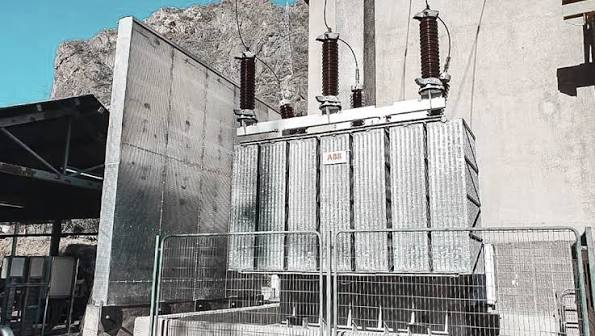
\includegraphics[width=\linewidth, height=4.3cm, keepaspectratio]{pictures/muro_corta_fuegos.jpeg}
      \caption{Muro cortafuego divisorio para transformador.}
    \end{subfigure}%
    \hfill
    \begin{subfigure}[b]{0.40\textwidth}
      \centering
      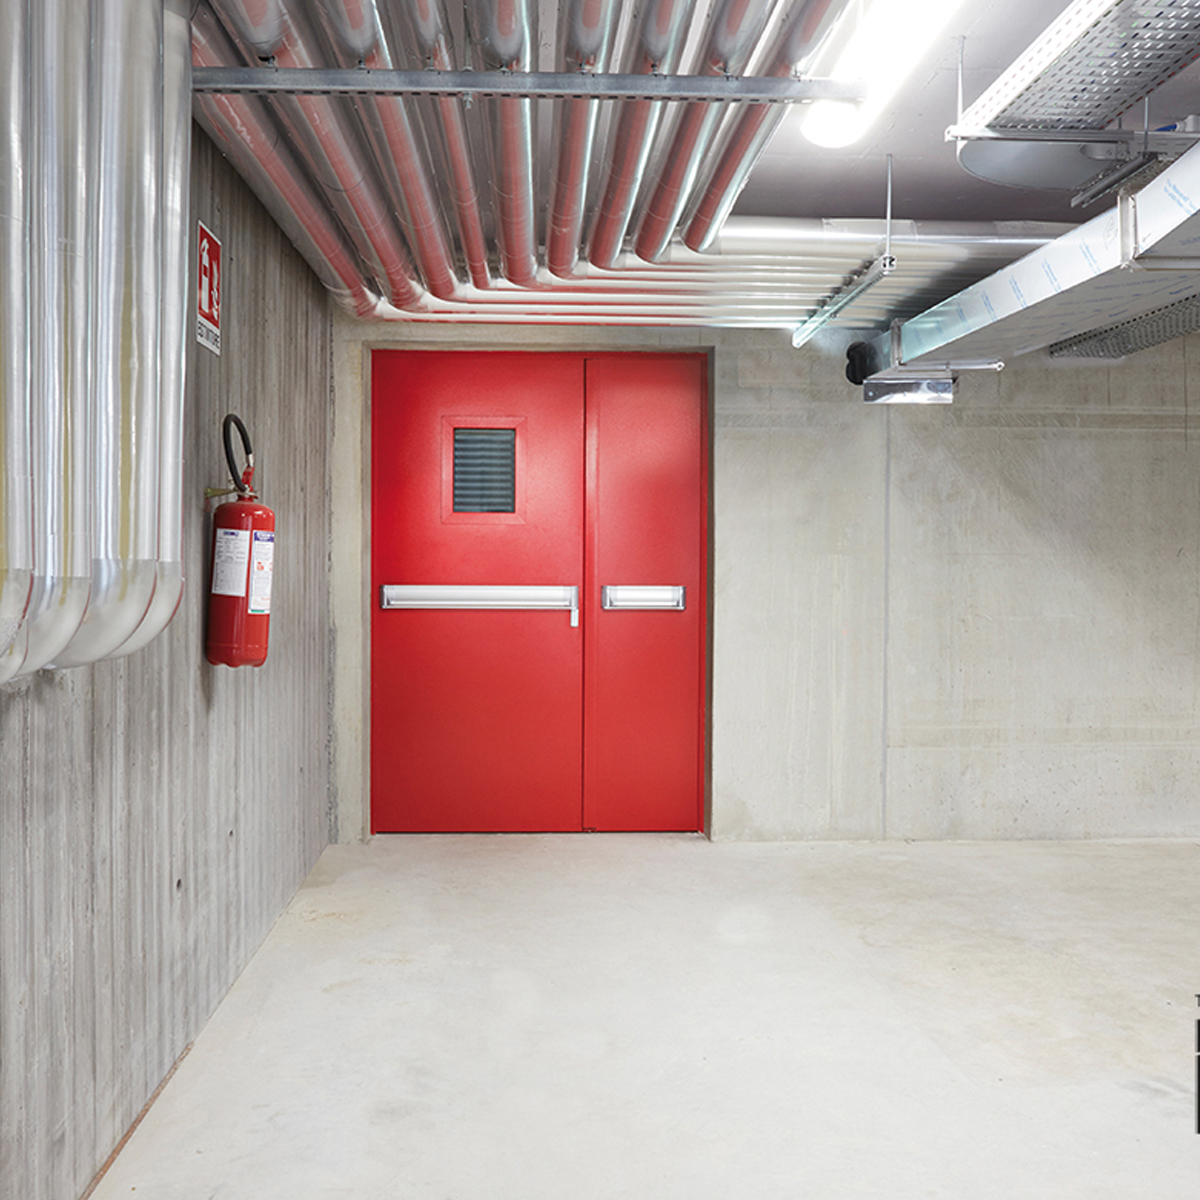
\includegraphics[width=\linewidth, height=4.3cm, keepaspectratio]{pictures/puertas-cortafuegos.jpg}
      \caption{Puertas cortafuego de doble contacto.}
    \end{subfigure}
  \end{figure}
\end{frame}


% --- SLIDE 51 (Pág 53 PDF): ESCALERAS PRESURIZADAS ---
\begin{frame}{Protección Pasiva: Cajas de Escalera Presurizadas para Evacuación}
  \begin{columns}[c]
    \begin{column}{0.50\textwidth}
      \small
      Garantía de rutas de escape libres de humos y gases tóxicos:
      \begin{itemize}
        \scriptsize
        \item En edificios industriales y corporativos, la caja de escaleras se convierte en chimenea de humos si se abre una puerta.
        \item \textbf{Presurización Mecánica Positiva:} Ventiladores de inyección forzada mantienen una sobrepresión continua de $\mathbf{50\,\mathrm{Pa}}$ dentro de la caja de escaleras.
        \item Cuando una puerta de escape se abre hacia la escalera, el gradiente de presión empuja el aire hacia afuera, impidiendo físicamente el ingreso de humos y gases calientes.
      \end{itemize}
    \end{column}

    \begin{column}{0.48\textwidth}
      \centering
      \resizebox{0.85\columnwidth}{!}{%
        \begin{tikzpicture}[scale=0.85]
          \draw[line width=1.5pt, fill=successgreen!10] (0,0) rectangle (2.2,3.5);
          \node[font=\scriptsize\bfseries, align=center] at (1.1,2.8) {Escalera\\$+50\,\mathrm{Pa}$};
          \draw[line width=1.5pt, fill=darkcharcoal!30] (2.2,0) rectangle (4.4,3.5);
          \node[font=\scriptsize\bfseries, align=center] at (3.3,2.8) {Piso con\\Fuego};
          \draw[->, >=stealth, line width=2pt, successgreen!80!black] (1.8,1.2) -- (2.6,1.2);
          \node[above, font=\tiny\bfseries] at (2.2,1.3) {Flujo de Aire Expulsa Humo};
        \end{tikzpicture}
      }
    \end{column}
  \end{columns}
\end{frame}

% --- PROTECCIÓN PASIVA/PREVENTIVA: SEÑALIZACIÓN ---
\begin{frame}{Protección Pasiva/Preventiva: Señalización}
  \begin{columns}[c]
    \begin{column}{0.46\textwidth}
      \small
      Sistema por el cual se facilita la evacuación aún en ausencia total de luz, indicando las salidas, salidas de emergencia, equipos de protección contra incendios, riesgos específicos, etc.
    \end{column}

    \begin{column}{0.52\textwidth}
      \centering
      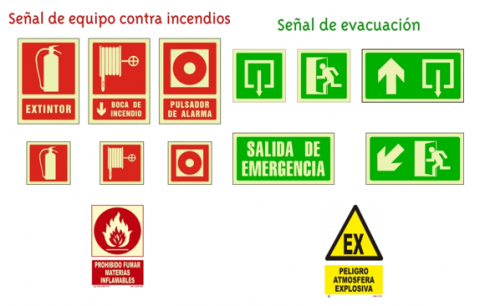
\includegraphics[width=\linewidth, keepaspectratio]{pictures/senalizacion_incendios.png}
    \end{column}
  \end{columns}
\end{frame}

% --- PROTECCIÓN PREVENTIVA: FUENTES DE IGNICIÓN E INSTALACIONES ---
\begin{frame}{Protección Preventiva: Fuentes de Ignición e Instalaciones}
  \begin{itemize}
    \small
    \item \textbf{Instalaciones eléctricas:} Tener en cuenta que la sección de los cables se adapte a la potencia instalada de los artefactos eléctricos a conectar, a fin de evitar cortocircuitos, líneas recargadas, etc.
    \item \textbf{Control de fuentes abiertas:} Apagar correctamente colillas de cigarrillos y fósforos.
    \item \textbf{Equipos térmicos:} Capacitar para el buen manejo de equipos industriales que producen calor y quemadores portátiles.
    \item \textbf{Corte y soldadura:} En trabajos de corte y soldadura mantener los locales ventilados.
    \item \textbf{Electricidad estática:} En operaciones que generen electricidad estática mantener la humedad elevada para evitarla.
  \end{itemize}
\end{frame}

% --- PROTECCIÓN PREVENTIVA: CONTROL DE COMBUSTIBLES Y RESIDUOS ---
\begin{frame}{Protección Preventiva: Control de Combustibles y Residuos}
  \begin{itemize}
    \small
    \item \textbf{Sustancias inflamables:} Almacenar los productos inflamables en lugares ventilados, rotulados y ubicarlos lejos de fuentes de calor.
    \item \textbf{Carga de fuego:} Evitar acumulación de residuos en áreas de trabajos para disminuir la carga de fuego.
    \item \textbf{Materiales y derivados:} Aplicar productos químicos
        ignifugantes, a la madera y sus productos o derivados.
    \item \textbf{Quema en planta:} Evitar la quema de residuos en la planta. Cuando la quema de residuos no pueda evitarse y sea admitida por el Organismo de control, es necesario:
    \begin{itemize}
      \footnotesize
      \item Limitar el lugar.
      \item Tener en cuenta el momento y las condiciones climáticas para hacerlo, y apagarlo cuando cambien las mismas, en especial, respecto al viento.
    \end{itemize}
  \end{itemize}
\end{frame}


% --- SLIDE 44 (Pág 46 PDF): ÉSTERES DIELÉCTRICOS ---
\begin{frame}{Protección Preventiva: Sustitución de Aceite}
  \begin{columns}[c]
    \begin{column}{0.70\textwidth}
      \small
      Riesgo de explosión en transformadores de potencia:
      \begin{itemize}
        \scriptsize
        \item \textbf{Aceite Mineral Convencional:} Hidrocarburo derivado del
            petróleo; punto de inflamación bajo ($140\text{ a }160\,\Celsius$).
              Un arco interno gasifica el aceite provocando fácilmente fuego Clase B.
        \item \textbf{Aceite vegetal o sintético:} Fluidos de clase K basados en
            aceites vegetales refinados o sintéticos:
        \begin{itemize}
          \tiny
          \item \textbf{Punto de fuego $> 300\,\Celsius$ a $> 360\,\Celsius$.}
          \item \textbf{Propiedad autoextinguible:} Si cesa el arco, la llama se extingue sin asistencia.
          \item Reduce drásticamente distancias de seguridad entre transformadores y elimina la necesidad de pesados muros cortafuego masivos.
        \end{itemize}
      \end{itemize}
    \end{column}

    \begin{column}{0.48\textwidth}
      \centering
      \resizebox{0.9\columnwidth}{!}{%
        \begin{tikzpicture}
          \draw[fill=firered!20, draw=firered, line width=1.2pt] (0,1.8) rectangle (4.2,3.2)
                node[midway, font=\scriptsize, align=center] {\textbf{Aceite Mineral}\\Punto Fuego $\approx 160\,\Celsius$\\Explosión violenta Clase B};
          \draw[fill=successgreen!20, draw=successgreen!80!black, line width=1.2pt] (0,0) rectangle (4.2,1.4)
                node[midway, font=\scriptsize, align=center] {\textbf{Aceite
                vegetal o sintético}\\Punto Fuego $> 300\,\Celsius$\\Autoextinguible $\cdot$ Biodegradable};
          \draw[->, >=stealth, line width=2pt, fireorange] (2.1,1.8) -- (2.1,1.4);
        \end{tikzpicture}
      }
    \end{column}
  \end{columns}
\end{frame}

% --- SLIDE 45 (Pág 47 PDF): DISPOSITIVOS AFDD ---
\begin{frame}{Protección Preventiva: Detección de Arco Serie AFDD (IEC 62606)}
  \begin{columns}[c]
    \begin{column}{0.52\textwidth}
      \small
      Límite de las protecciones tradicionales ante arcos serie:
      \begin{itemize}
        \scriptsize
        \item Un conductor fisurado o un borne flojo genera microarcos eléctricos en serie intermitentes.
        \item La corriente de arco en serie está limitada por la propia carga del circuito; \textbf{nunca supera la corriente nominal} ($I_{\mathrm{falla}} < I_n$).
        \item En consecuencia, \textbf{termomagnéticas y disyuntores diferenciales no actúan}.
        \item \textbf{Solución AFDD:} Microcontrolador que analiza la forma de
            onda de la corriente. En caso de detección de anomalía abre el
              circuito rápidamente.
      \end{itemize}
    \end{column}

    \begin{column}{0.45\textwidth}
      \centering
      \resizebox{0.82\columnwidth}{!}{%
        \begin{tikzpicture}[scale=0.8]
          \draw[line width=1pt, ->] (0,0) -- (4.5,0) node[right, font=\tiny] {$t$};
          \draw[line width=1pt, ->] (0,-1.4) -- (0,1.6) node[above, font=\tiny] {$i(t)$};
          % Onda senoidal distorsionada con ruido en el cruce
          \draw[line width=1.2pt, utnblue] (0,0) 
                .. controls (0.5,1.5) .. (1.0,1.2) 
                -- (1.2,0.8) -- (1.3,1.1) -- (1.4,0.7) 
                .. controls (1.8,-0.2) .. (2.2,0)
                .. controls (2.7,-1.5) .. (3.2,-1.2)
                -- (3.4,-0.8) -- (3.5,-1.1) -- (3.6,-0.7)
                .. controls (4.0,0) .. (4.2,0);
          \node[above, font=\tiny\bfseries, firered] at (1.3,1.2) {Ruido RF de Arco};
        \end{tikzpicture}
      }\\[4pt]
      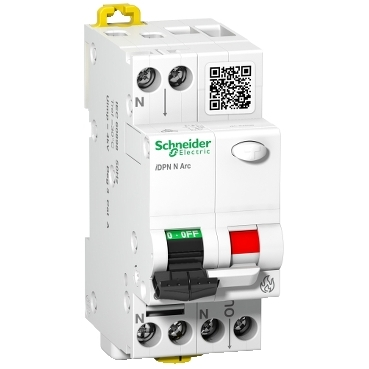
\includegraphics[height=3.0cm, keepaspectratio]{pictures/AFDD.jpg}
    \end{column}
  \end{columns}
\end{frame}

% --- SLIDE 46 (Pág 48 PDF): TERMOGRAFÍA INFRARROJA ---
\begin{frame}{Protección Preventiva: Mantenimiento Predictivo por Termografía}
  \begin{columns}[c]
    \begin{column}{0.50\textwidth}
      \small
      Diagnóstico fallas de origen térmico en tableros:
      \begin{itemize}
        \scriptsize
        \item El aflojamiento mecánico por vibraciones o fatiga térmica genera un aumento de la resistencia en los puntos de contacto.
        \item Por ley de Joule ($P = I^2 R_c$), el borne se calienta progresivamente hasta degradar el aislamiento plástico.
        \item \textbf{Inspección Termográfica Calibrada:} Relevamiento con cámara infrarroja bajo carga nominal del establecimiento.
        \item Gradientes térmicos $\Delta T \ge 10\,\Celsius$ respecto a conductores sanos determinan la intervención preventiva con parada programada.
      \end{itemize}
    \end{column}

    \begin{column}{0.48\textwidth}
      \centering
      \resizebox{0.85\columnwidth}{!}{%
        \begin{tikzpicture}
          \draw[fill=darkcharcoal!20, draw=darkcharcoal, line width=1.2pt] (0,0) rectangle (3.5,2.4);
          \fill[firered] (1.75,1.2) circle (0.5);
          \fill[yellow] (1.75,1.2) circle (0.25);
          \node[font=\tiny\bfseries, white] at (1.75,1.2) {$85\,\Celsius$};
          \node[below, font=\tiny\bfseries] at (1.75,0.4) {Punto Caliente en Borne};
        \end{tikzpicture}
      }
    \end{column}
  \end{columns}
\end{frame}

% --- SLIDE 52: BRIGADAS EPI Y ESI ---
\begin{frame}{Organización Humana de Respuesta: E.P.I. y E.S.I.}
  \small
  Estructura escalonada para la gestión humana de emergencias (doctrina de cátedra y SRT):

  \vspace{0.4cm}
  \centering
  \begin{tikzpicture}[
    line cap=round, line join=round,
    boxcomite/.style={draw=darkcharcoal, fill=cardbg, line width=1.3pt, rounded corners=5pt, text width=7.4cm, align=center, inner sep=6pt},
    boxepi/.style={draw=firered, fill=firered!12, line width=1.3pt, rounded corners=5pt, text width=5.7cm, align=center, inner sep=6pt},
    boxesi/.style={draw=utnblue, fill=utnblue!12, line width=1.3pt, rounded corners=5pt, text width=5.7cm, align=center, inner sep=6pt}
  ]
    % Comité (arriba centro)
    \node[boxcomite] (Comite) at (0, 1.8) {
      {\small\textbf{\textcolor{darkcharcoal}{Comité de Emergencia y Jefe de Emergencia}}}\\[3pt]
      {\scriptsize Conducción estratégica $\;\cdot\;$ Orden de evacuación $\;\cdot\;$ Punto de encuentro}
    };

    % EPI (abajo izquierda)
    \node[boxepi] (EPI) at (-3.65, -0.8) {
      {\small\textbf{\textcolor{firered}{Equipo de Primera Intervención (E.P.I.)}}}\\[3pt]
      {\scriptsize Fuerza de choque en taller $\;\cdot\;$ Advertencia\\[2pt] Extintores en $<30\,\mathrm{s}$}
    };

    % ESI (abajo derecha)
    \node[boxesi] (ESI) at (3.65, -0.8) {
      {\small\textbf{\textcolor{utnblue}{Equipo de Segunda Intervención (E.S.I.)}}}\\[3pt]
      {\scriptsize Brigada de planta $\;\cdot\;$ Mangueras $45/63.5\mm$\\[2pt] ERA $\;\cdot\;$ Bomberos}
    };

    % Conexiones jerárquicas desde Comité
    \coordinate (fork) at (0, 0.5);
    \draw[line width=1.3pt, darkcharcoal] (Comite.south) -- (fork);
    \draw[->, >=stealth, line width=1.3pt, darkcharcoal] (fork) -| (EPI.north);
    \draw[->, >=stealth, line width=1.3pt, darkcharcoal] (fork) -| (ESI.north);

    % Coordinación operativa entre EPI y ESI
    \draw[<->, >=stealth, line width=1.3pt, dashed, darkcharcoal!80] (EPI.east) -- (ESI.west);

  \end{tikzpicture}
\end{frame}

% --- SLIDE 43: JERARQUÍA DE CONTROL DE RIESGOS ---
\begin{frame}{La Jerarquía de Control de Riesgos (ISO 45001 / IRAM 3800)}
  \begin{columns}[c]
    \begin{column}{0.48\textwidth}
      \small
        Jerarquía de medidas según efectividad (de mayor a menor prioridad):
      \begin{enumerate}
        \scriptsize
        \item \textbf{Eliminación:} Suprimir físicamente el peligro en el diseño.
        \item \textbf{Sustitución:} Reemplazar reactivos y fluidos combustibles por alternativas no inflamables.
        \item \textbf{Controles de Ingeniería:} Salvaguardas tecnológicas automáticas, AFDD, termografía, ventilación forzada.
        \item \textbf{Controles Administrativos:} Protocolos de trabajo seguro, permisos PTC y metodología 5S.
        \item \textbf{EPP:} Atenuación del impacto residual sobre el trabajador.
      \end{enumerate}
    \end{column}

    \begin{column}{0.50\textwidth}
      \centering
      \resizebox{0.95\columnwidth}{!}{%
        \begin{tikzpicture}[yscale=0.7]
          \draw[fill=firered!80, line width=1pt] (0,4) rectangle (5.4,4.7) node[midway, text=white, font=\scriptsize\bfseries] {1. Eliminación};
          \draw[fill=fireorange!80, line width=1pt] (0.3,3) rectangle (5.1,3.7) node[midway, text=white, font=\scriptsize\bfseries] {2. Sustitución};
          \draw[fill=amberyellow!85!black, line width=1pt] (0.6,2) rectangle (4.8,2.7) node[midway, text=white, font=\scriptsize\bfseries] {3. Controles de Ingeniería};
          \draw[fill=utncyan, line width=1pt] (0.9,1) rectangle (4.5,1.7) node[midway, text=white, font=\scriptsize\bfseries] {4. Controles Administrativos};
          \draw[fill=utnblue, line width=1pt] (1.6,0) rectangle (3.8,0.7) node[midway, text=white, font=\scriptsize\bfseries] {5. EPP};
        \end{tikzpicture}
      }
    \end{column}
  \end{columns}
\end{frame}

% --- SLIDE 53: CASO IRON MOUNTAIN ---
\begin{frame}{Análisis Forense: Depósito Iron Mountain (Barracas, 2014)}
  \begin{columns}[c]
    \begin{column}{0.50\textwidth}
      \small
      Lecciones del colapso estructural de Barracas:
      \begin{itemize}
        \scriptsize
        \item \textbf{Carga de fuego extrema ($Q_f \gg 150\,\kg/\m^2$):} Racks metálicos autoportantes de más de $10\,\m$ densamente cargados de papel.
        \item \textbf{Efecto tiro de chimenea vertical:} Aceleración violenta de las llamas hacia el techo.
        \item \textbf{Falla activa total:} Válvulas de rociadores cerradas sin presurización; bombas principales apagadas.
        \item \textbf{Ausencia de protección pasiva en el acero:} Al superar los $900\,\Celsius$, el acero sufrió fluencia térmica, pandeó y empujó el muro este hacia la calle Jovellanos, provocando el fallecimiento de 10 rescatistas.
      \end{itemize}
    \end{column}

    \begin{column}{0.48\textwidth}
      \centering
      \resizebox{0.85\columnwidth}{!}{%
        \begin{tikzpicture}
          \draw[line width=1.5pt, fill=firered!10] (0,0) rectangle (3.5,3.0);
          \draw[line width=2pt, dashed, firered] (0,0) -- (-0.8,2.8) node[above, font=\tiny\bfseries, firered] {Colapso hacia la calle};
          \node[font=\tiny\bfseries, align=center] at (1.75,1.5) {Fluencia térmica a $>900\,\Celsius$\\Pandeo de cabriadas\\Empuje sobre muro exterior};
        \end{tikzpicture}
      }
    \end{column}
  \end{columns}
\end{frame}

% --- SLIDE 54: CASO EDESUR CABALLITO ---
\begin{frame}{Análisis Forense: Subestación Edesur Caballito (2024)}
  \begin{columns}[c]
    \begin{column}{0.50\textwidth}
      \small
      Falla durante mantenimiento electromecánico:
      \begin{itemize}
        \scriptsize
        \item Intervención sobre transformador de $132/13.2\,\mathrm{kV}$ con máquina de filtrado de aceite caliente.
        \item Rotura de manguera flexible bajo presión: pulverización de aceite mineral sobre bornes calientes/energizados.
        \item \textbf{Fuego mixto Clase B + Clase C:} Propagación inmediata por túneles y bandejas de cables aislados con PVC convencional.
        \item Columnas densas de humo negro y $HCl$ bloquearon la visibilidad y demoraron el ataque.
        \item \textbf{Lección de diseño:} Obligatoriedad de ésteres dieléctricos autoextinguibles y conductores LS0H en subestaciones urbanas.
      \end{itemize}
    \end{column}

    \begin{column}{0.48\textwidth}
      \centering
      \resizebox{0.85\columnwidth}{!}{%
        \begin{tikzpicture}
          \draw[fill=darkcharcoal!20, line width=1.2pt] (0,0) rectangle (3.2,2.2) node[midway, font=\tiny\bfseries] {Transformador de Potencia};
          \draw[->, >=stealth, line width=2pt, firered] (3.2,1.1) -- (4.2,1.1) node[right, font=\tiny\bfseries, firered] {Fuga de Aceite};
          \node[below, font=\tiny\bfseries] at (1.6,-0.2) {Propagación por cables de PVC};
        \end{tikzpicture}
      }
    \end{column}
  \end{columns}
\end{frame}

% --- SLIDE 55: MATRIZ RESUMEN Y CONCLUSIONES ---
\begin{frame}{Matriz Síntesis de Soluciones y Conclusiones Finales}
  \small
  La prevención y protección eficaz conforma un sistema integral de barreras múltiples:

  \vspace{0.2cm}
  \begin{table}[h]
    \centering
    \scriptsize
    \begin{tabular}{p{2.8cm} p{2.2cm} p{3.4cm} p{3.2cm}}
      \toprule
      \textbf{Medida de Solución} & \textbf{Nivel / Tipo} & \textbf{Mecanismo Técnico} & \textbf{Impacto Operativo} \\
      \midrule
      \textbf{Ésteres Dieléctricos} & Sustitución / Prev. & Punto de fuego $>300\,\Celsius$, autoextinguible & Elimina explosión Clase B en transformadores. \\
      \addlinespace
      \textbf{Cables LS0H} & Sustitución / Prev. & Poliolefinas sin halógenos; vapor no tóxico & Mantiene visibilidad y evita corrosión de silicio. \\
      \addlinespace
      \textbf{Dispositivos AFDD} & Ingeniería / Prev. & Detección de firma de RF de arco serie & Evita arcos que burlan a termomagnéticas. \\
      \addlinespace
      \textbf{Sectorización $F$} & Ingeniería / Pasiva & Muros certificados y sellos intumescentes & Confinamiento físico del fuego y gases calientes. \\
      \addlinespace
      \textbf{Brigadas E.P.I. / E.S.I.} & Humana / Activa & Advertencia precoz y ataque con hidrantes & Ataque en $<30\,\mathrm{s}$ y enlace con bomberos. \\
      \bottomrule
    \end{tabular}
  \end{table}
\end{frame}

% =============================================================================
% CIERRE: AGRADECIMIENTOS Y RONDA DE PREGUNTAS
% =============================================================================

\begin{frame}[standout]
  \Huge\textbf{¡Muchas Gracias!}\\[0.6cm]
  \normalsize\textbf{Espacio abierto para preguntas, consultas y comentarios}\\[0.5cm]
  \scriptsize
  \textbf{Disertantes (Comisión 4R2):}\\
  Ignacio Gil $\cdot$ Gaston Grasso $\cdot$ Franco Palombo $\cdot$ Angelo Prieto\\[0.2cm]
  \textit{Universidad Tecnológica Nacional --- Facultad Regional Córdoba}\\
  \textit{Cátedra de Seguridad, Higiene y Medio Ambiente}
\end{frame}


\end{document}
